\documentclass[11pt]{article}
\usepackage[utf8]{inputenc}
\usepackage{amsmath,amssymb}
\usepackage{graphicx}
\graphicspath{ {./images/} }
\usepackage[margin = 1.3 in]{geometry}
\usepackage{titlesec}
\usepackage{textcomp}
\usepackage{sidecap}
\usepackage{verbatimbox}
\sidecaptionvpos{figure}{t}
\usepackage{wrapfig}
\usepackage[margin=0cm]{caption}
\captionsetup[figure]{labelfont={bf},name={Figure},font=footnotesize}
\usepackage{multicol}
\usepackage{enumitem}
\pagenumbering{gobble}



\begin{document}
\begin{titlepage}
    \title{\vspace{40pt}\Huge KiriZen: Creation of a Kirigami Inspired iPhone Application in Swift}

    \author{ \\\hline \\\\\\ \Large \vspace{5pt} Author: Stephanie Tindal \\\Large \vspace{5pt}{Student ID: 1936508}\\\Large \vspace{50pt}{Supervisor: Achim Jung} \\ \hline\\\\\\  \vspace{5pt}{MSc Computer Science} \\ \vspace{5pt}{School of Computer Science, University of Birmingham}\\\\\\ \hline\\\\}

    \date{September 2019 \vspace{20pt}}
    \maketitle

\end{titlepage}
    \tableofcontents
\newpage

\begin{abstract}
    This project focuses on creating an iPhone application inspired by kirigami and designed to create a relaxing immersive experience. Kirigami is a paper cutting art derived from origami where paper is folded and shapes are cut out of it, resulting in symmetrical patterns when unfolded. I conducted background research by investigating similar applications to gain an understanding of the market I would be designing an app for. I then expanded my idea and took it through development by first creating two generations of prototypes, which were critiqued by prospective users. The application involves two activities, creating a cutting pattern from a virtually folded piece of paper, and attempting to match a target pattern which has been randomly selected. The application was implemented in Swift. The decisions involved in creating the core functionality are discussed, in addition to the human computer interaction aspects of the application. Nielsen's heuristics were used to evaluate the final application. Although I faced considerable challenges and limitations during production, which I have discussed, I was able to meet the aim of this project, and successfully create a kirigami app, KiriZen.

\end{abstract}

\vspace{50pt}
\renewcommand{\abstractname}{Acknowledgements}
\begin{abstract}
    I would like to thank Professor Achim Jung for supervising me throughout the project and Dr Iain Styles for the initial idea of an origami based application. 
\end{abstract}

\newpage

\section{Introduction}
\pagenumbering{arabic}

        \subsection{A Brief Introduction to Origami and Kirigami}
        
            \paragraph{}
            Origami is the art of folding paper. One of its earliest depictions was the folding of an ancient Egyptian map made from papyrus. Upon the invention of paper, origami was used mainly in religious ceremonies due to its high price. Origami is evidenced to be used by many cultures, with the exact time point of invention unclear.\cite{origamiBible}
            
            After folding paper became popular, cutting followed. Cutting paper transcends many cultures. Scherenschnitte is the German and Swiss art of cutting paper which produces intricate silhouettes \cite{Scherenschnitt}. ``Papel picado", meaning perforated paper, is created in Mexico and hung in the streets as banners for celebration \cite{GlobalPaperCutting} and paper cuttings are created for the Jewish holiday Shavuot \cite{CJNews}. Kirigami, in addition to origami, includes cutting the paper. In Japanese, ``kiru'' means ``to cut" \cite{Temko2004kirigami} and ``kami" means paper \cite{WordHippo}. The word ``kirigami" was created by Florence Temko and popularised by her book ``Kirigami, the Creative Art of Papercutting" \cite{OrigamiResourceCenter}. Kirigami was initially used in religious ceremonies in Japan representing elegance and wealth. It is still used today in many religious festivals and recreationally \cite{kyuhoshiInfo}. The famous magician Harry Houdini describes many origami and kirigami designs in his book ``Houdini’s Paper Magic". One example of a design used as a magic trick is folding a square piece of paper into a triangular shape and using one straight cut with scissors to create a five point star \cite{PaperMagic}. Today kirigami is an activity commonly used across many cultures at Christmas to make snowflakes.
            
            \subsubsection{Relevance}
                \paragraph{}
                Origami and kirigami are becoming more common in pop culture. Fashion has been inspired by kirigami, illustrated by Nida Azwer's entire collection dedicated to Kirigami at Pakistan Fashion Week 2016 \cite{NidaAzwer}.
                Alexandra Verschueren won the L'Oréal Professional Grand Prize at the Hyères International Festival of Fashion and Photography with her unique innovative designs inspried by kirigami \cite{AlexandraVerschueren}. Nahoko Kojima is a kirigami artist whose collections have been displayed in numerous locations worldwide, most recently in the Dulwich Picture Gallery in London featuring a 8.5m crocodile \cite{NahokoKojima}.
                Kanako Yaguchi is another artist who will have her 2019 kirigami exhibition displayed in Tokyo \cite{KanakoYaguchi}. In addition, Marc Hagan-Guirey is a paper artist who gained popularity with the creation of the Star Wars kirigami book which displays how to create models inspired by the movies \cite{StarWars}.
            
                Kirigami is also utilised in a scientific context. The cuts and folds of kirigami can be used to turn 2D structures into 3D structures that do not cause materials to fracture and allow some elasticity. Therefore, these structures can be used to create membranes of silicon or metal for nanostructured biomedical devices.\cite{MedicalTextures}.%Edit medical bit 
                Recently a medical device has been created which is essentially a  plastic ribbon that is sliced with cuts inspired from kirigami which allows it to twist. These twists in turn revealed microscopic twists in tissue that can be used to identify biological tissues when radiation was guided thorough these ribbons \cite{MedicalDevice}.
               These examples show how kirigami can be creatively used to produce innovative devices.
               
               In recent years, relaxation and mindfulness activities and applications (apps) are growing in popularity amongst all age groups. Such stress relieving activities include colouring, origami and app guided meditation. This has led me to the idea of creating a kirigami themed application for the purpose of creativity and relaxation.
    
            \subsection{Project Aim}
            
                 \paragraph{} 
                 
                  Having been a keen creator of origami from the age of 4, it was suggested by one of my professors that I create an application that involves origami. Upon discussion with my supervisor we decided the focus should be on kirigami. 
                  
                  The aim of the project is to create an application whereby users can create cuts in a virtually folded sheet of paper. The application will then reveal the unfolded pattern to them upon the click of a button. The application will include another activity which prompts the users to match a target pattern. The user will need to imagine how to cut the target shown from the folded piece of paper.
                  
                  In both activities, the paper should be folded an even number of times (2, 4, 6, or 8). You cannot fold a piece of paper into odd numbers about a centre point which is why they are excluded here.
                  
                  Despite the increased popularity of meditative applications, only a handful of applications based on kirigami were found during my research. Therefore, I believe there is a gap in the market which this application could fill.


                  \subsection{Swift}
               
                \paragraph{} 
                    I decided to create an iPhone application as this was an area of software development I had not yet explored and wanted to develop my skills in a new programming language. To create iPhone applications, Swift is a common language to use (with some Objective-C still being used on occasion) and Xcode is the integrated development environment (IDE) used for Swift. In order to learn Swift, I completed Udemy courses \cite{Udemy} on the basics of the language and the IDE. 
                   
                    I predicted that I would encounter some difficulties, due to my unfamiliarity with front-end coding and the fact that many methods have different names to those in Java.
                
               % despite some similarites in the language
               
               

\newpage
\section{Background Research}

        \subsection{Kirigami-like Applications}
           \paragraph{}
            I searched for applications on the web and Apple app store (specifically iPhone apps compatible with iPhone 7/8) with a theme that centered around creating kirigami. I chose the most popular and relevant applications that came up when I typed in key words such as ``Kirigami", ``cut", ``paper" in different combinations. I wanted to gain an insight into what is already available to ensure that my idea was unique, and to evaluate the strengths and weaknesses of the other apps as a user to learn from them before I began designing my own app.
            
            \subsubsection{Paper Snowflake Maker}
            
                \paragraph{Type:} Web application \cite{PaperSnowflakeMaker}
                \paragraph{Description:}
                Paper Snowflake Maker is a website where the user can cut out polygons from the shape of a folded piece of paper by clicking on the screen to make the corners of the polygon (right panel in \textbf{Figure~\ref{fig:paperSnowflakeMaker}}). The paper snowflake is virtually created and revealed to the user (left panel in \textbf{Figure~\ref{fig:paperSnowflakeMaker}}).
                    \begin{figure}[ht]\centering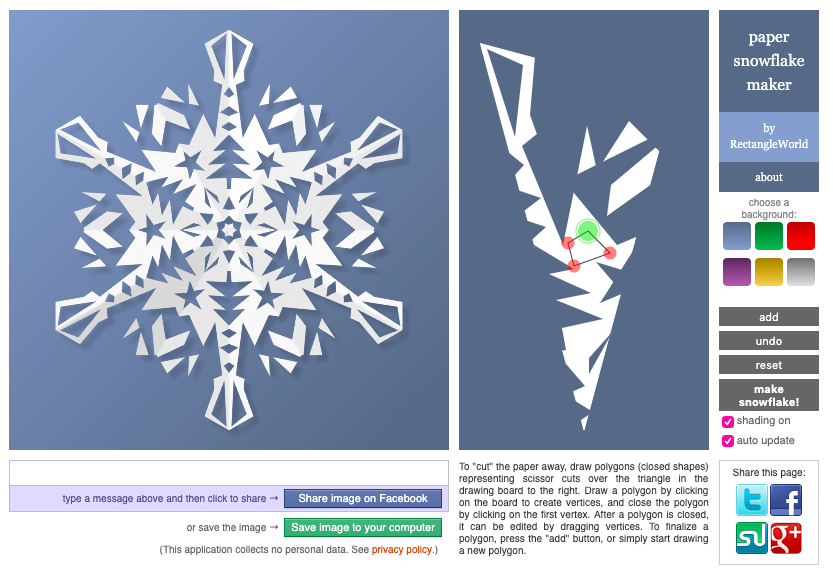
\includegraphics[width=0.9\textwidth]{Images/paperSnowflakeMaker}
                        \caption{
                        \label{fig:paperSnowflakeMaker}
                        A full page screenshot taken from the web application Paper Snowflake Maker. The user has made cuts on the folded image and is about to complete their next cut. The green dot indicates the beginning of a cut, the red dots indicate the corners of the polygon to be cut. When the users mouse passes over the green dot, an additional circle is created around its edge indicating to the user that if they click there, the polygon they created will be cut from the virtual piece of paper (the latter scenario is illustrated in this figure). The corners of the polygon can be dragged to a different shape before the cut is finalised.}
                    \end{figure}
                    
                \paragraph{Strengths:}
                It is clear how to make cuts in the virtually folded piece of paper as soon as you click on it, as seen on the right panel in \textbf{Figure~\ref{fig:paperSnowflakeMaker}}. The green and red dots that appear as you click are clear indicators for the progression of the cut.
                
                The auto update button is a convenient feature as the user does not have to click the ``make snowflake!" button every time a new shape is cut. 
                
                The draggable corners are an additional convenient feature if the user would like to edit the shape of the polygon before the cut is created.
                 
                 The shading of the final snowflake provides a sense of reality as its shadows appear in the same way as folded piece of paper.
                 
                \paragraph{Weaknesses:}
                When using the application, the add button (which finalises the cut, removing the construction lines on the folded paper image) seems unnecessary as it has the same functionality as other actions, such as starting to draw a new shape, or clicking the ``make snowflake!" button.
                
                The cuts that can be made on this virtual snowflake are much more complex than those which can be recreated on a real piece of paper, to some extent, this undermines the sense of realism indicated by the accurate shadows of the folds. The smaller pieces that are created in \textbf{Figure~\ref{fig:paperSnowflakeMaker}} would fall off after being severed from the main larger component also affecting the realism.
                
                The ``Save image to your computer" button opens another window explaining how to save the image (using ``Save Image As...") which is unnecessary and ironically the user is not able to save the image on their computer via this pop-up window. Copying the image produced a low resolution image, as does saving the image straight from the original screen. In addition, the ``Share image on Facebook" button does not work.
            
                \paragraph{Lessons Learned:}
                The cutting is intuitive for this web application, I can consider this approach when developing my own cutting method. The overall look of the application is clean, however, the buttons on the side and instructions could be updated for a more modern feel and rearranged to improve the user experience. Buttons that do not provide the intended functionality should be discarded (such as the ``Save image to your computer" button).
                
            \subsubsection{Snowflake!}
            
                \paragraph{Type:} iPhone application \cite{Snowflake}
            
                \paragraph{Description:}
                Snowflake! is an application that allows the user to cut out free-form shapes from either 22.5\textdegree{} segments (four folds creating eight repeating shapes) or 45\textdegree{} segments (eight folds creating sixteen repeating shapes). The image revealed is a snowflake-like shape as shown in \textbf{Figure~\ref{fig:snowflakeResult}} which is created from the 22.5\textdegree{} segments in \textbf{Figure~\ref{fig:snowflakeSegmentCut}}. 
                    
                    \begin{figure}[!ht]
                        \begin{minipage}{0.45\textwidth}
                            \centering 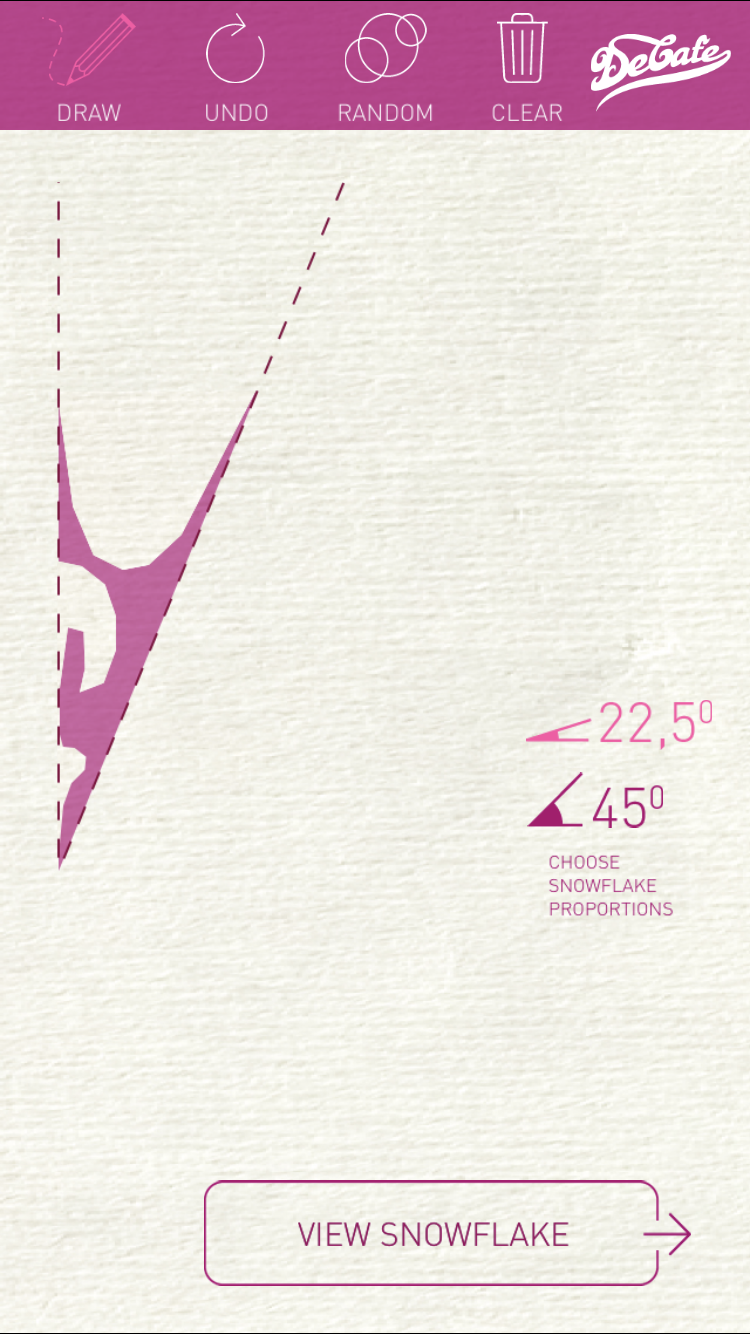
\includegraphics[width=0.7\linewidth]{Images/snowflakeSegmentCut}
                            \caption{A ready made cut resulting from the ``Random" button. The segment size selected is 22.5\textdegree{}. Pressing the ``View Snowflake" button takes the user to the screen in \textbf{Figure~\ref{fig:snowflakeResult}}.\\}
                            \label{fig:snowflakeSegmentCut}
                        \end{minipage}\hfill
                        \begin{minipage}{0.45\textwidth}
                            \centering
                            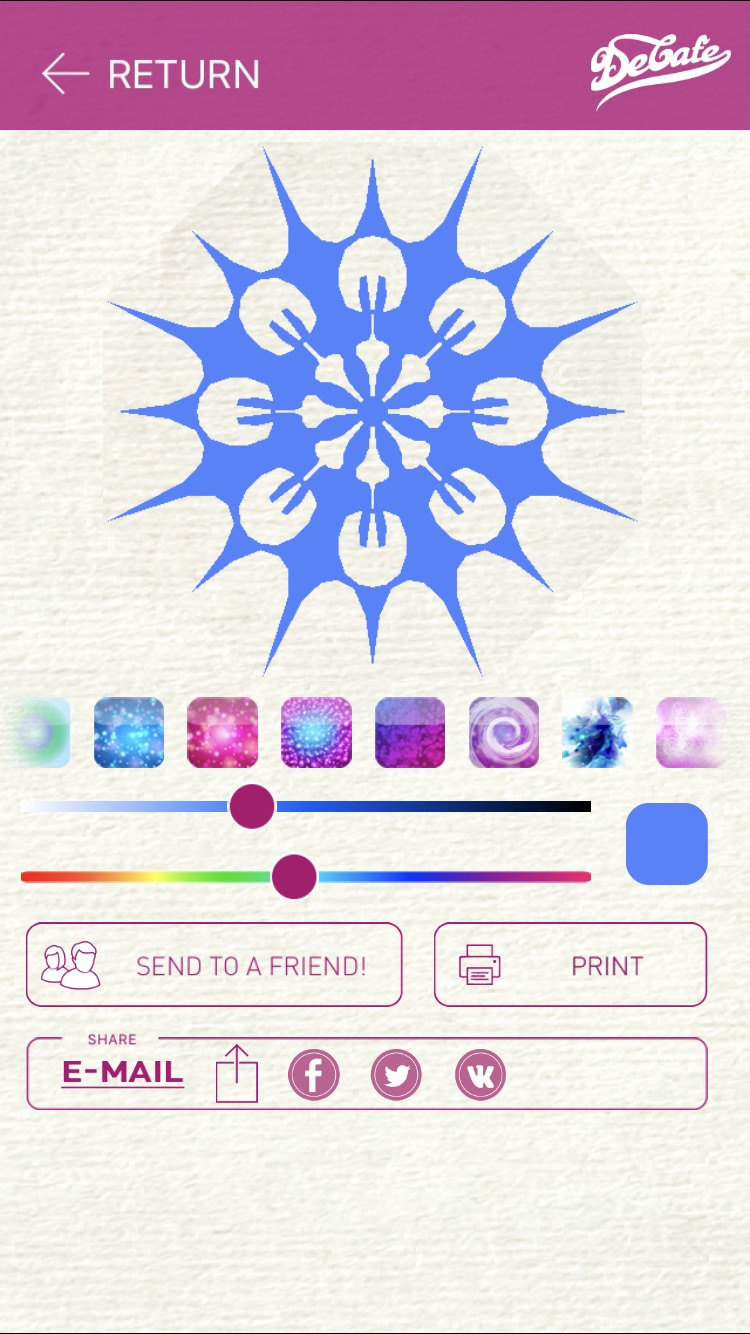
\includegraphics[width=0.7\linewidth]{Images/snowflakeResult}
                            \caption{The result of the cut made in \textbf{Figure~\ref{fig:snowflakeSegmentCut}}. The colour of the image can be altered with the colour pickers below it. The image can be shared with the buttons in the ``Share" section providing the relevant button works.}
                            \label{fig:snowflakeResult}
                        \end{minipage}
                    \end{figure}
                    
                \paragraph{Strengths:}
                A version of Tchaikovsky's ``Dance of the Sugar Plum Fairy" plays in the background which is synonymous with Christmas in keeping with the theme of the application. 
                The user can use the random shape button to create a base to start with. The user can change the colour scheme of the snowflake if desired.
                
                \paragraph{Weaknesses:}
                Snowflakes have six sides due to the shape of the H\textsubscript{2}O molecule. Eight sided crystals would never be formed naturally therefore it is an odd choice for this application to choose pieces of paper folded into segments with angles of 22.5\textdegree{} and 45\textdegree{}, as this forms eight or sixteen sided snowflakes rather than the more common six or at most twelve sided snowflakes \cite{H2O}. 
                
                The area of the screen dedicated to the main function of creating cuts from a segment of the final shape consists of a very small portion of the screen. The ratio is especially low when cutting from the 22.5\textdegree{} segments as seen in \textbf{Figure~\ref{fig:snowflakeSegmentCut}}.
                
                The shape that is cut from the shape drawn is not always as expected. For example, in \textbf{Figure~\ref{fig:snowflakeOutline}} this does not reflect the cut you would expect from the free-form shape drawn by the user in \textbf{Figure~\ref{fig:snowflakeCut}}.
               
                On the share bar displayed in the centre of \textbf{Figure~\ref{fig:snowflakeResult}}, the ``Send to a friend!" button has exactly the same response as the ``E-Mail" button. It is also slightly  misleading as I would expect this button to create a message via WhatsApp or iMessage rather than email if sending to a friend. The upload icon button allows the user to create a ``Happy new year" themed postcard. When the ``Send" button is pressed, the pop-up disappears, leaving the user uncertain as to where the image they just created was saved or sent. Unlike with the buttons that do work, the user is sent to the relevant email or social media screen. The same situation occurs when the Twitter button (icon of a bird) is pressed, and no response occurs after the ``Send" button is pressed.
                The status bar disappears on the app so the user is not able to see information such as signal, battery life time etc while using the application. 
                 
                 \begin{figure}[!ht]
                        \begin{minipage}{0.45\textwidth}
                            \centering 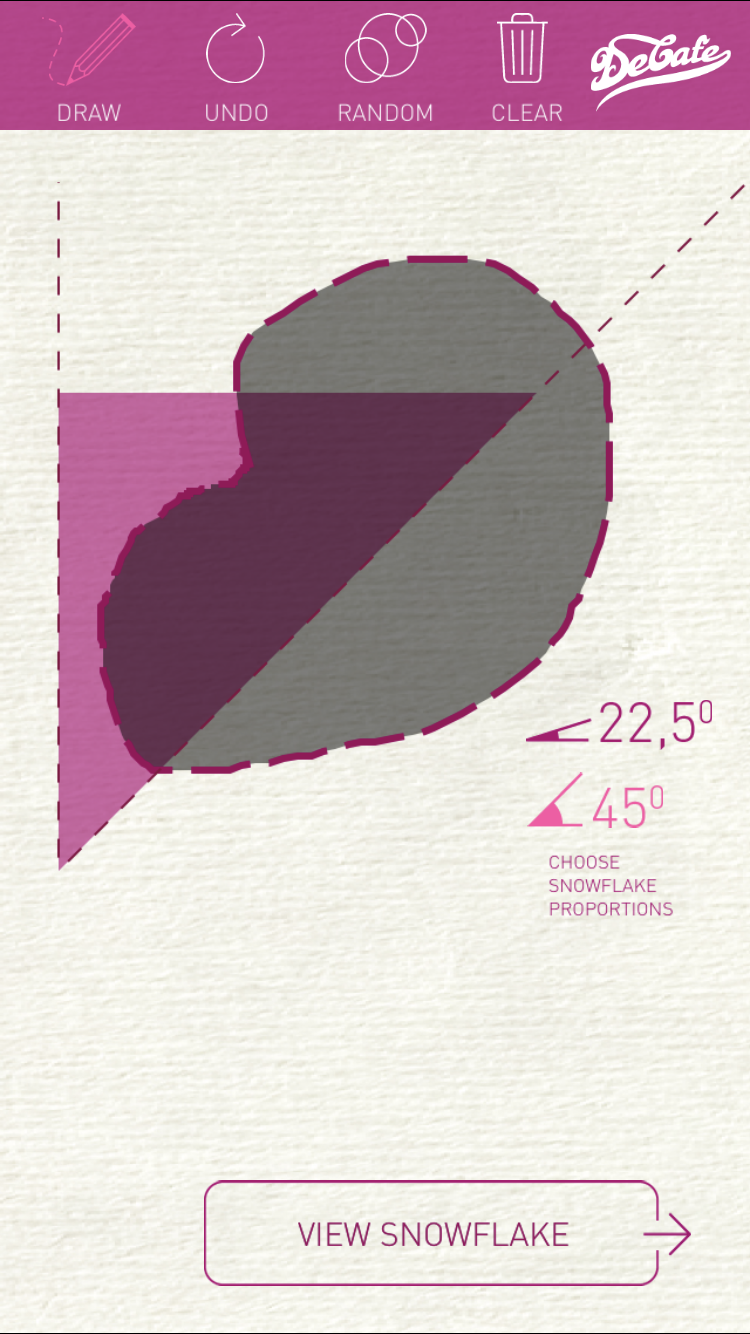
\includegraphics[width=0.7\linewidth]{Images/snowflakeOutline}
                            \caption{A free-form line is drawn on a 45\textdegree{} segment to indicate where the user has drawn the cut.\\\\}
                            \label{fig:snowflakeOutline}
                        \end{minipage}\hfill
                        \begin{minipage}{0.45\textwidth}
                            \centering
                            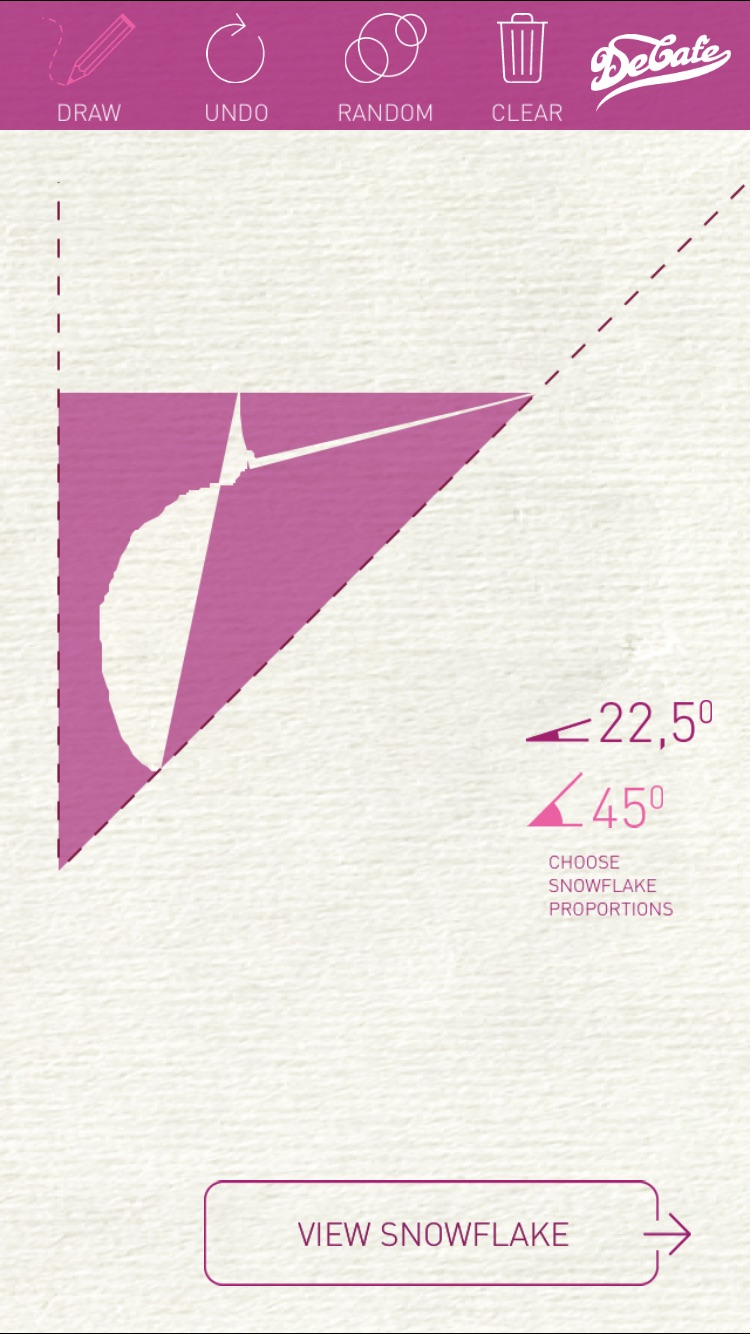
\includegraphics[width=0.7\linewidth]{Images/snowflakeCut}
                            \caption{The result of the free-form line drawn in \textbf{Figure~\ref{fig:snowflakeOutline}}. There is a bug in the application as this is not the cut the user would expect from what they have drawn.}
                            \label{fig:snowflakeCut}
                        \end{minipage}
                    \end{figure}
        
                \paragraph{Lessons Learned:}
                An application should be researched before it is made and assumptions should be checked, such as the assumption made about the dimensions of a snowflake. If the functionality of the buttons in the app are not working, there should be a response message from the application to inform the user of what the problem is. Each button should have unique functionality. The cuts that are to be made in the virtual piece of paper should take up a large portion of the screen, as this is the main area the user is interacting with.
            
            
            \subsubsection{Kirie}
            
                \paragraph{Type:} iPhone application \cite{Kirie}

                \paragraph{Description:}
                This application allows the user to draw lines (which are transformed into cuts) on a virtual piece of paper folded in half vertically. The virtual piece of paper is unfolded upon reveal. 

                \paragraph{Strengths:}
                The majority of the screen is used when creating the cut. This allows you to make intricate cuts and the overall feel of the app is minimalistic. 
                
                It is possible for a user to upload their own images to use in the application, either as a background image, or to cut from.
                
                 \begin{wrapfigure}{r}{0.25\textwidth}
                    \centering
                    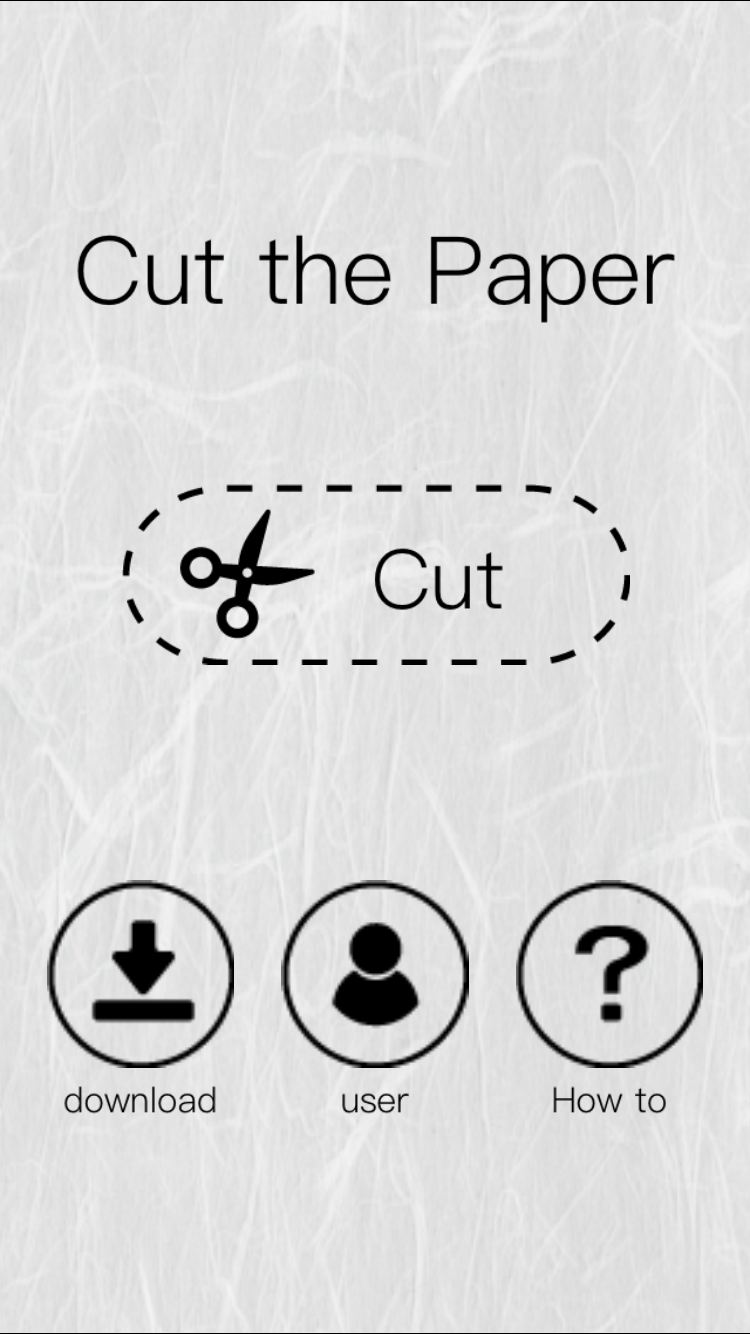
\includegraphics[width=0.25\textwidth]{Images/kirieMain}
                    \captionsetup{{margin = 0.2cm}}
                    \caption{The home screen of the Kirie app. The three buttons at the bottom of the screen either cause the app to crash or do not provide their proposed functionality. Only the ``Cut" button has the expected action of taking the user to the next screen.}
                    \label{fig:kirieMain}
                \end{wrapfigure}
                
                
                \paragraph{Weaknesses:}
                On the initial screen (seen in \textbf{Figure~\ref{fig:kirieMain}}), only the ``Cut" button works. It is also not very clear that the ``Cut" button is a button, it could easily be  mistaken for a logo, especially as the other buttons of the screen are of a different format. There is also no highlight or shading response for the button which can cause further confusion. This is a particular problem in this case as the reaction to the button is slow. If the ``download" button is pressed, the app crashes and closes. If the ``How to" button is pressed, there is no response from the app. If the ``user" button is pressed, a pop up shows up prompting a username. With any input the application closes the popup and returns to the same screen as before. There also appears no way to sign up or login. It should also be noted that the captions for the buttons do not have consistent capital letters to start (``How to" does, the other buttons do not), a minor flaw that shows lack of attention to detail.
                
                On the finished cut screen shown in \textbf{Figure~\ref{fig:kirieCut}} the save icon button does not save the image anywhere, despite a confirmation pop-up. It is unclear what the functionality of the picture icon button is, as the cuts have already been finalised. The upload icon results in a confirmation pop-up (saying the image has been uploaded) but no upload has actually occurred, the user was not even asked where they would like the image to be uploaded. 
                
                The trace from the user's finger is very sensitive and can result in cuts that are not smooth. The same shape cut, such as the top and bottom ``X" created in \textbf{Figure~\ref{fig:kirieXs}}, results in two cuts seen in \textbf{Figure~\ref{fig:kirieCut}}. Firstly these cuts are not consistent with those that would occur with a cutting knife or scissors, therefore making it difficult for the user to predict what the shape of the cut will be from the lines they draw. Secondly similar lines result in different cuts due to the starting point of each line.
                
                \begin{figure}[!ht]
                        \begin{minipage}{0.45\textwidth}
                            \centering 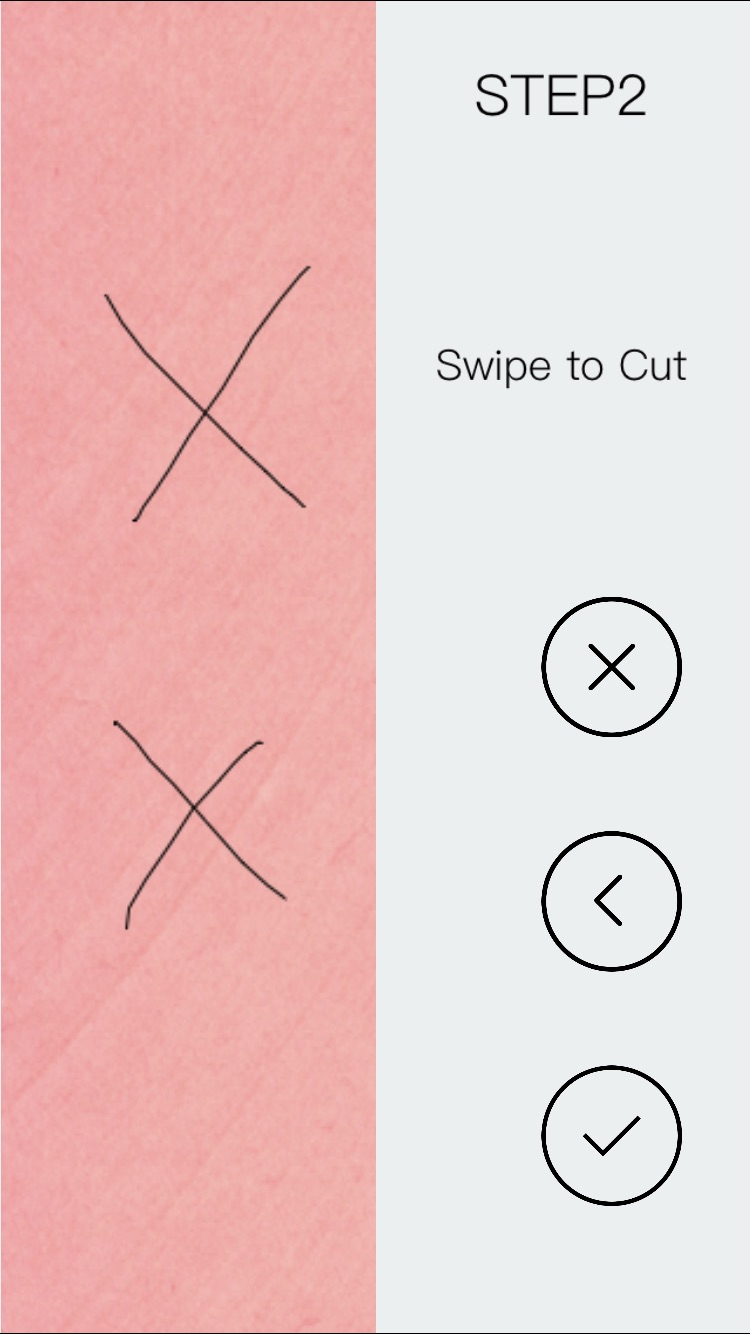
\includegraphics[width=0.7\linewidth]{Images/kirieXs}
                            \caption{The lines drawn by the user on the left panel. The top ``X" although it looks very similar to the bottom ``X" produces a different cut as shown in  \textbf{Figure~\ref{fig:kirieCut}}.\\\\}
                            \label{fig:kirieXs}
                        \end{minipage}\hfill
                        \begin{minipage}{0.45\textwidth}
                            \centering
                            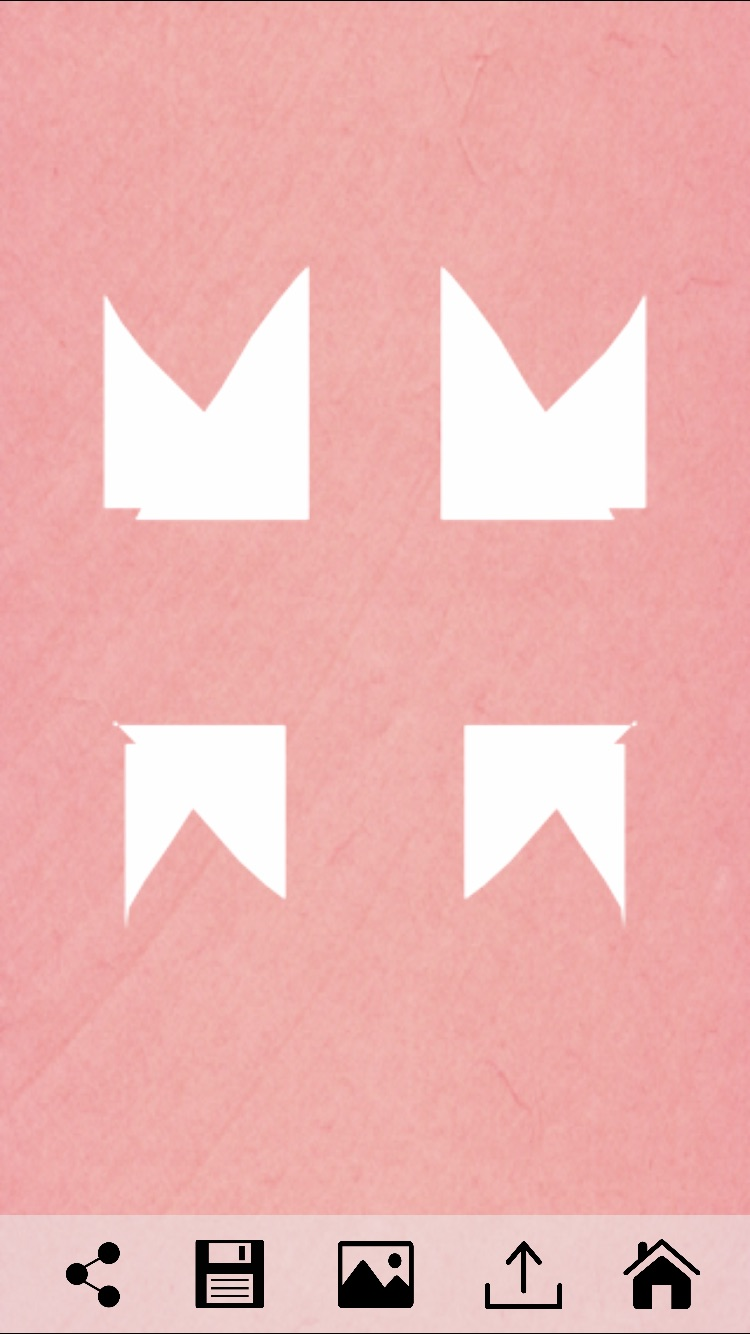
\includegraphics[width=0.7\linewidth]{Images/kirieCut}
                            \caption{The result of the ``X"s drawn in \textbf{Figure~\ref{fig:kirieXs}}. The right hand side is a reflection of the left. The cuts are not what would be expected from the ``X" lines drawn and the results for each X would be more similar rather than a reflected shape.}
                            \label{fig:kirieCut}
                        \end{minipage}
                    \end{figure}
                
                \paragraph{Lessons Learned:}    %check paragraphs
                A large portion of the screen allows the user to have more control thus facilitating a greater space for creativity.
                
                It is useful to have all the buttons of a similar format for the application so they can all be recognised and used correctly.
                
                The cuts created do not have to be closed shapes resulting in unexpected shapes being created after the user confirms the cut. The application should restrict the user to only create closed shapes as that would allow them to predict where the cuts would be made resulting from their line. When the cuts are mirrored, the resolution of the image of the cuts decreases. %(add a connective to this last sentence)
               
                If the functionality of the buttons causes the application to crash, this is a major error and is unacceptable for any application. All buttons should be thoroughly tested throughout creation of my application. There could be confirmation pop-ups in my application but only when the functionality works, unlike in ``Kirie".
                
                The variety of tasks to do in the app is very limited. Overall, the usefulness of the app is questionable as it just reflects the cuts in the y-axis and there is no other reflection or folding option. Additional features that add little to the app and are somewhat unnecessary or relevant should not be implemented. Any unessential features should be added after the main functionality of the application works well.
                
                
                 \subsubsection{Handcraft Snowflakes}
            
                \paragraph{Type:} iPhone application \cite{PeppaHippo}

                \paragraph{Description:}
                This application uses the character of Peppa Hippo, similar to Peppa Pig, a British children's cartoon character, throughout. The application consists of cutting shapes out of a segment of a snowflake. There is a gallery available where your snowflakes can be saved. Coins can either be purchased or collected whilst using the app. They are redeemed for new ready made shapes to cut the snowflake with, new background textures/colours for the snowflake paper, or to add pages in the gallery booklet for saving more snowflakes. 

                \paragraph{Strengths:}
                The theme is consistent through the use of a character. Some of the audience for Peppa Hippo may be directed to this application on the App store. There are many language options enabling the character of Peppa Hippo to speak in the selected language. A large proportion of the screen dedicated to cutting shapes from the snowflake. In this case the snowflake has a reasonable number of sides. 

                \begin{wrapfigure}{r}{0.25\textwidth}
                    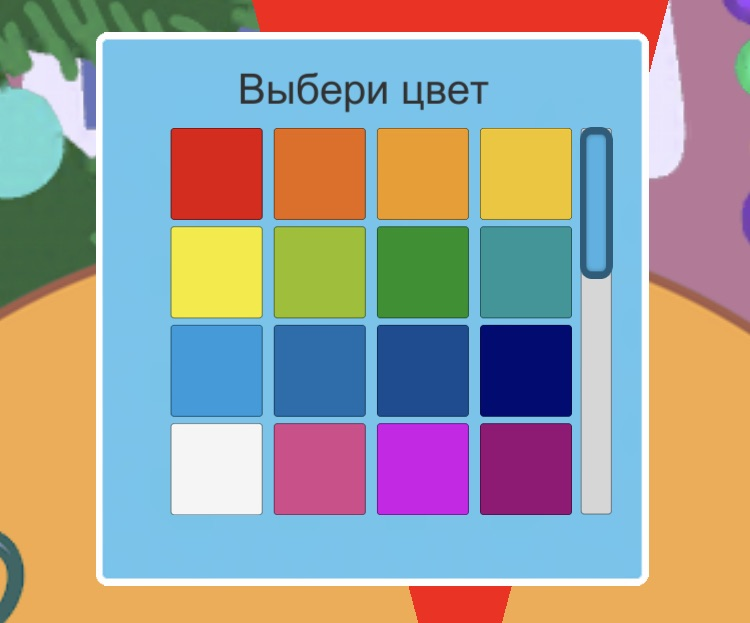
\includegraphics[width=0.25\textwidth]{Images/peppa/peppaRussian}
                    \captionsetup{{margin = 0.2cm}}
                    \caption{The current language selected is Spanish, however the colour picker has a title in Russian.}
                    \label{fig:peppaRussian}
                \end{wrapfigure}
                \paragraph{Weaknesses:}
                The commentary by Peppa Hippo does not contain much helpful information on how to use the app, it merely states the obvious such as ``Let's start making a snowflake". The character's name is not in the title of the application, this means there is less exposure to the Peppa Hippo audience.
                
                Even after selecting a language, its use is not consistent throughout the application. For example, no matter which language you pick, the title for some sections, for example the colour picker is always displayed in Russian as seen in \textbf{Figure~\ref{fig:peppaRussian}}.  As the application is clearly aimed at children this may be confusing for them unless they understand Russian. 
                
                There is a black loading page before every screen is displayed which stops the flow of the app and makes the app feel slow.

                \begin{figure}[!ht]
                        \begin{minipage}{0.32\textwidth}
                            \centering 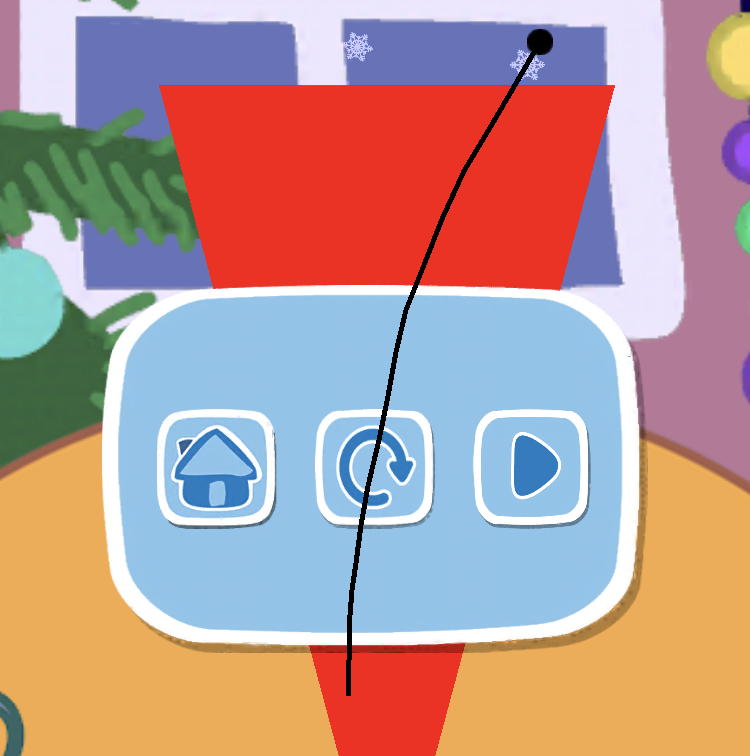
\includegraphics[width=0.8\linewidth]{Images/peppa/peppaGlitchLine}
                            \captionsetup{{margin = 0.2cm}}
                            \caption{The user can still interact with the line on the screen despite the exit screen pop-up being displayed. This can make the action the user wishes to carry out feel ambiguous.}
                            \label{fig:peppaGlitchLine}
                        \end{minipage}
                        \begin{minipage}{0.32\textwidth}
                            \centering
                            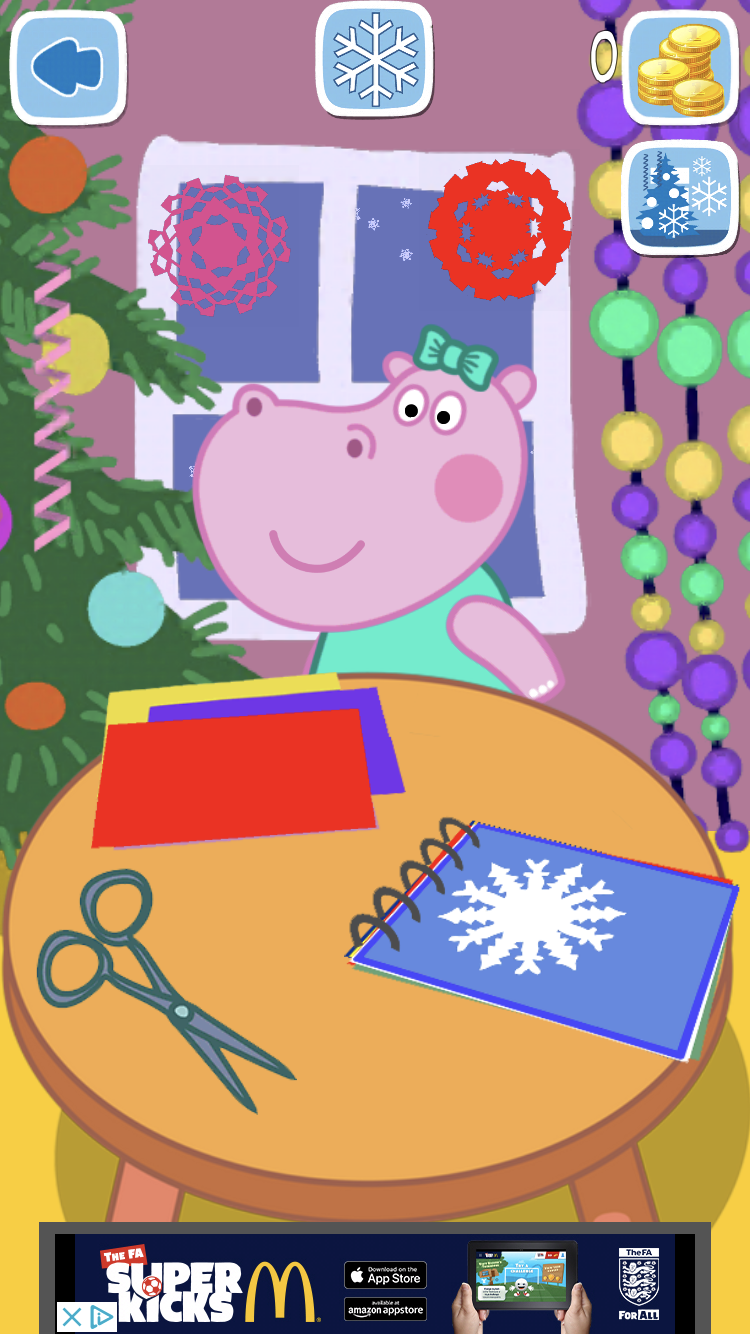
\includegraphics[width=0.8\linewidth]{Images/peppa/peppaMain}
                             \captionsetup{{margin = 0.2cm}}
                             \caption{The main screen where users can select the coloured paper to cut snowflakes, or the notepad to view their snowflake gallery.\\}
                            \label{fig:peppaMain}
                        \end{minipage}
                        \begin{minipage}{0.32\textwidth}
                            \centering
                            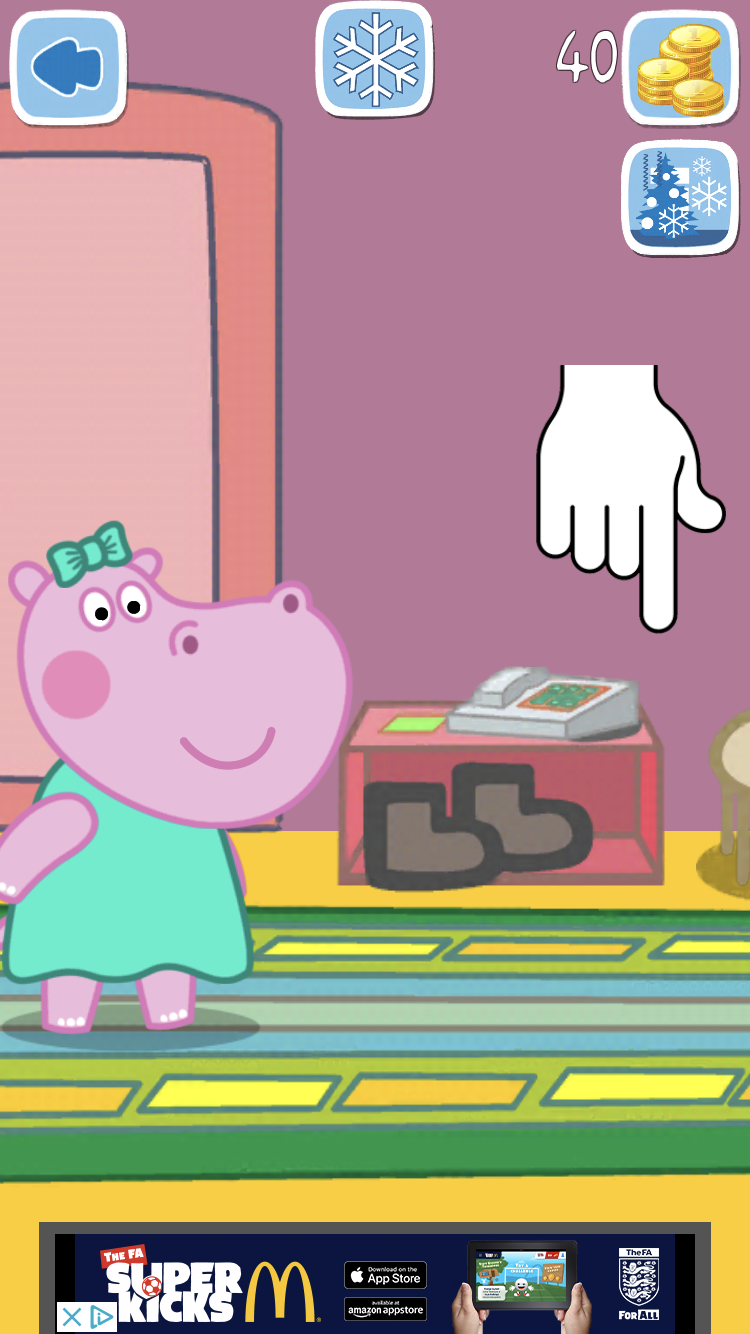
\includegraphics[width=0.8\linewidth]{Images/peppa/peppaGlitchPoint}
                             \captionsetup{{margin = 0.2cm}}
                             \caption{A hand appears on screen prompting the user to interact with the phone or shoes. This is misleading the user as they cannot interact with any object in the current frame.}
                            \label{fig:peppaGlitchPoint}
                        \end{minipage}
                    \end{figure}
                    
                    There are glitches on the free-form creation screen displayed in \textbf{Figure~\ref{fig:peppaGlitchLine}}. Cuts can still be made on the paper via the underlying view when a pop up is displayed. This should be disabled and the line should be displayed in the layer below the pop up.
                
                    It is unclear which objects can be interacted with throughout the application. For example, in \textbf{Figure~\ref{fig:peppaMain}} the scissors would be the most obvious object to interact with to start cutting the snowflakes, however the user can only interact with the coloured paper and the notepad. On occasion there appears to be a glitch illustrated in \textbf{Figure~\ref{fig:peppaGlitchPoint}} where the application indicates to the user an item should be tapped, however in fact none of the objects in the frame are interactive. 
                    
                    \begin{figure}[!ht]
                        \begin{minipage}{0.32\textwidth}
                            \centering 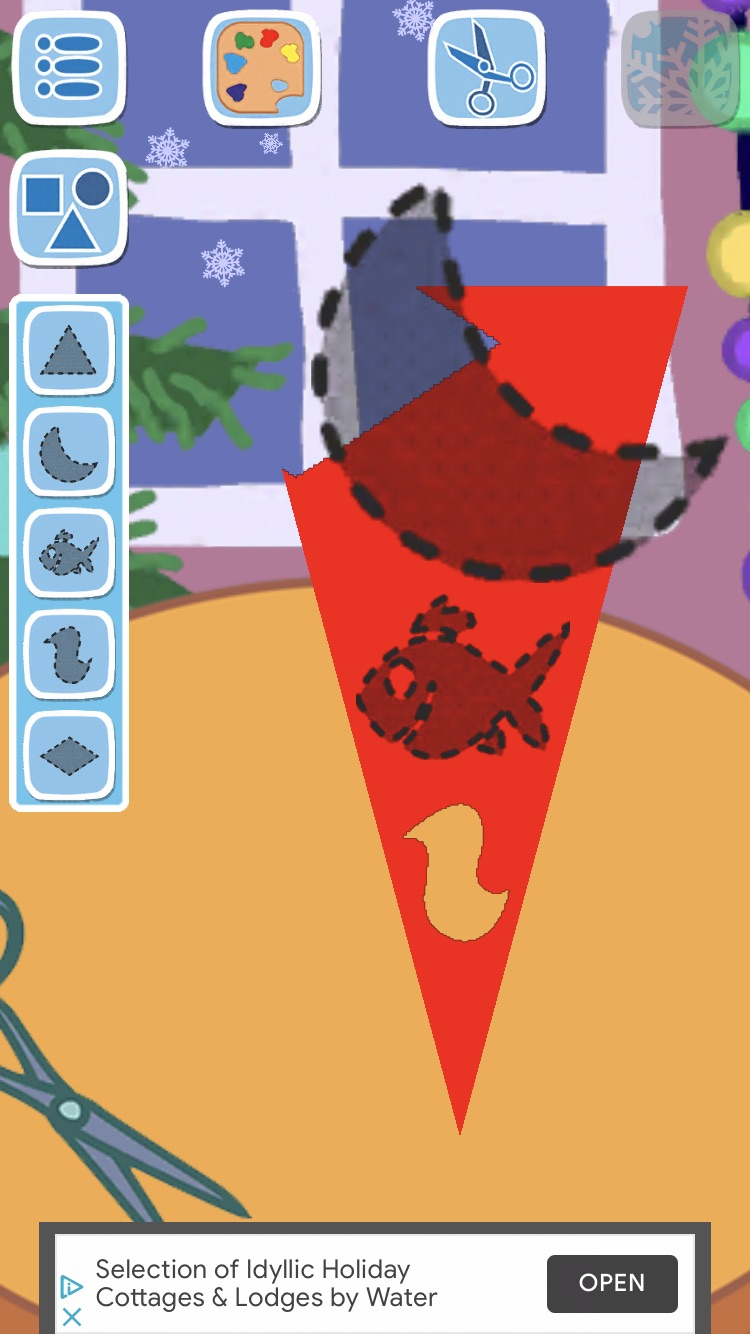
\includegraphics[width=0.8\linewidth]{Images/peppa/peppaShapes}
                            \captionsetup{{margin = 0.2cm}}
                            \caption{The user can drag and drop shapes onto the paper, resizing the shapes if desired. There is the option to pick more shapes if the button with multiple shapes is pressed.}
                            \label{fig:peppaShapes}
                        \end{minipage}
                        \begin{minipage}{0.32\textwidth}
                            \centering
                            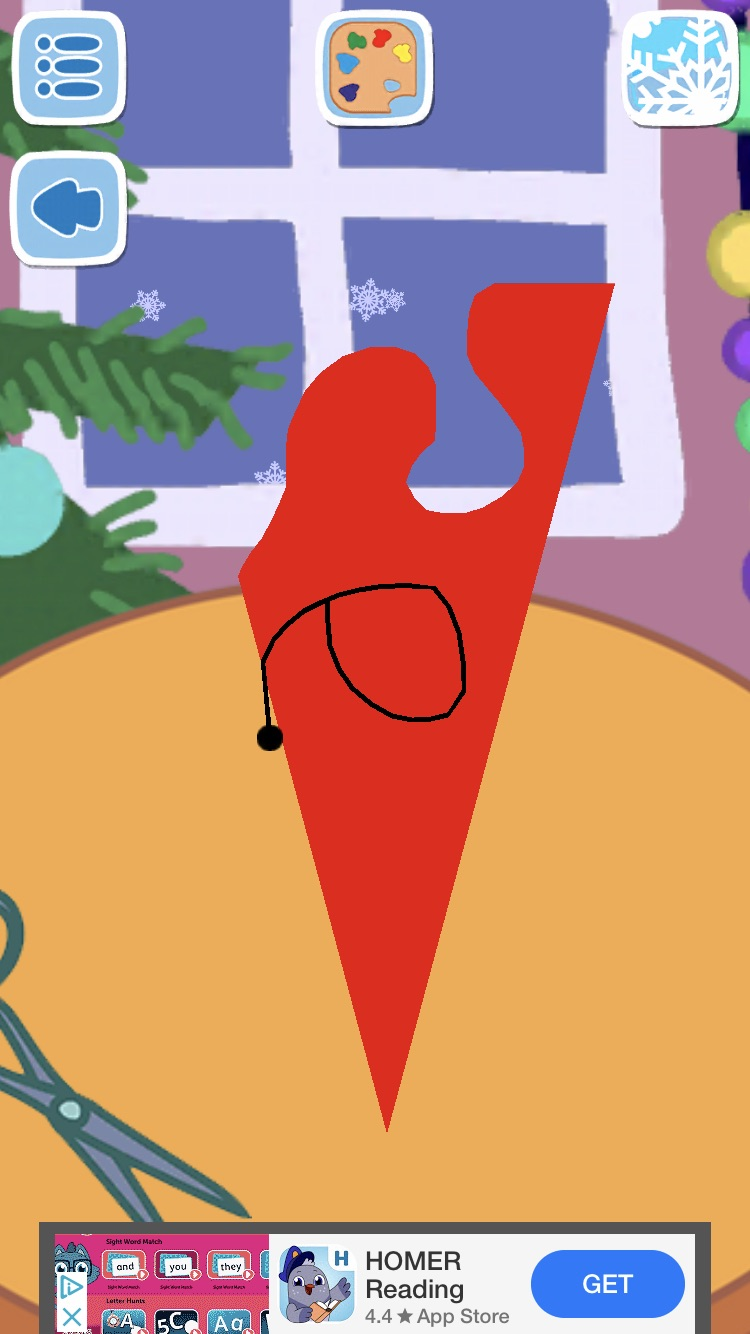
\includegraphics[width=0.8\linewidth]{Images/peppa/peppaFreeFormCut}
                             \captionsetup{{margin = 0.2cm}}
                             \caption{The user is able to create free-form cuts with their finger on this screen. Many glitches occur with the free-form cut creation page of the app.}
                            \label{fig:peppaFreeFormCut}
                        \end{minipage}
                        \begin{minipage}{0.32\textwidth}
                            \centering
                            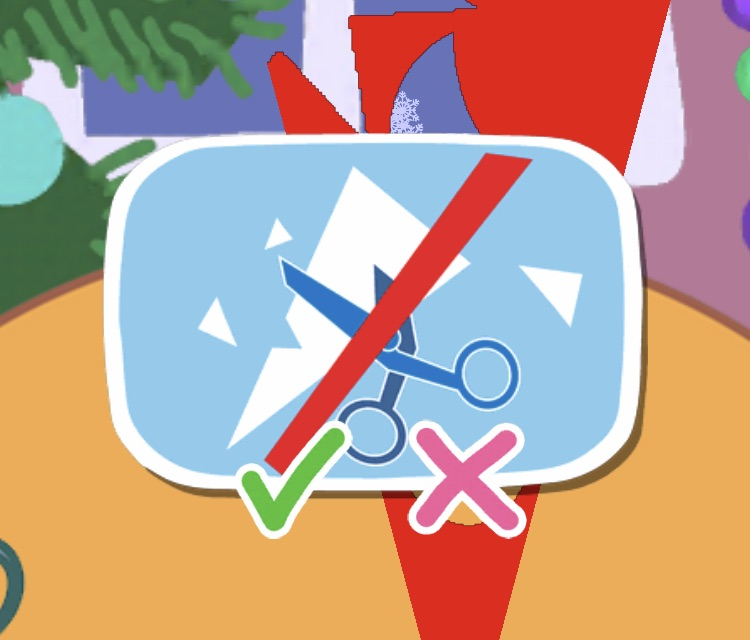
\includegraphics[width=0.8\linewidth]{Images/peppa/peppaPopUp}
                             \captionsetup{{margin = 0.2cm}}
                             \caption{This pop-up is usually displayed if a button that will exit the creation screen is pressed. It is unclear whether the tick is prompting the user to keep the snowflake or remove it.}
                            \label{fig:peppaPopUp}
                        \end{minipage}
                    \end{figure}
                    
                    The app will freeze if the cutting line comes in contact with itself as shown in \textbf{Figure~\ref{fig:peppaFreeFormCut}}. Sometimes the paper is not cut, even when the line the user is drawing is registered. If the user moves their finger too quickly, the cut may not be created and the registered line will disappear as if an illegal cut was drawn.
                    
                    On the ready made shapes page (\textbf{Figure~\ref{fig:peppaShapes}}), it is not obvious that you need to drag the shapes of the cuts as they appear in the same location as the button bar. They only appear if you drag your finger not when you tap the button (even though the button will flash indicating something should happen). 
                    
                    The ready made cuts produce a jagged edge if the user enlarges them as seen in cut made in the top left of \textbf{Figure~\ref{fig:peppaShapes}}. Some of the ready made cuts are not in keeping with the theme such as duck and fish shapes for a snowflake / Christmas application. 
                    The main problem with the application is the assumed knowledge of the buttons. For example, in \textbf{Figure~\ref{fig:peppaMain}} and \textbf{Figure~\ref{fig:peppaGlitchPoint}} it is unclear what the buttons with snowflakes on them in will do. They appear to allow the user to drag snowflakes onto the window in the background, however, it is difficult to use so the functionality is unclear. The left facing arrow button on the main screen shown in \textbf{Figure~\ref{fig:peppaMain}} will take the user back to the previous screen. This navigation to a previous screen is a common action for the left arrow button. However, on the free-form cut screen shown in \textbf{Figure~\ref{fig:peppaFreeFormCut}}, pressing the left arrow button will undo the shape the user has just cut.
                 On the shape cutting screen, there is no undo option for cuts made. There is a lack of consistency with the image of the button making use of the application unnecessarily complex.
                
                The adverts are very distracting to the user's experience. The theme of Peppa Hippo limits the audience to children. 
                
                The animation still continues to speak when the mute button within the application or on the phone itself is activated, and the user cannot skip the animation. A pop-up (\textbf{Figure~\ref{fig:peppaPopUp}}) occurs if a button is pressed which will exit the user from the cutting screen, however it is unclear which button to press to continue working on the shape or to discard it. Also, since multiple buttons activate this pop-up, it occurs very frequently, adding to the disruption.
                
                The name of the application is too long for the icon, therefore you cannot see the entire name of the app on iPhone screen only ``Handcraft:S...".
                
                \paragraph{Lessons Learned:}   
                Additional features such as sound, language and animation should not detract from the application experience. Instead, these features should enhance the experience and only do so when the core features work well already. 
                
                Using images for buttons is tricky. It is done well in some cases, for example, the colour picker button uses a paint palette in \textbf{Figure~\ref{fig:peppaShapes}}, but not in others. For example, in \textbf{Figure~\ref{fig:peppaMain}} the function of the buttons with a snowflake on is unclear. It should be obvious whether the user can interact with images throughout the application. Consistency with buttons is key.
                
        \subsection{Cutting Paper Applications}
            \subsubsection{Paper Cut Craft}
            
                \paragraph{Type:} iPhone application \cite{PaperCutCraft}
                
                \paragraph{Description:} This application is for cutting a piece of paper into the target shape. 
                
                \paragraph{Strengths:}
                The cutting feature can be quite realistic at times. The line follows the users touch and is generally quite smooth. After a cut is made, the paper has an animation where the cut half falls off which is a good additional feature.
                
                \begin{wrapfigure}{r}{0.25\textwidth}
                    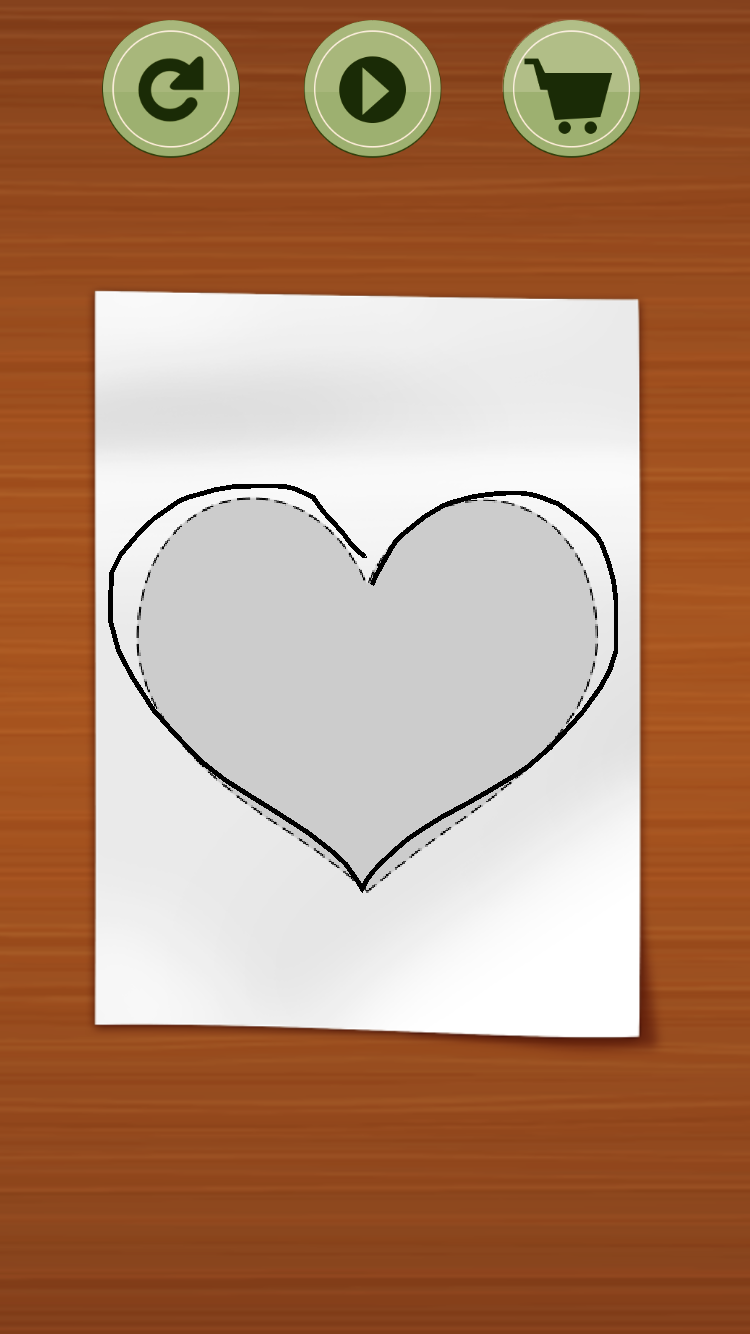
\includegraphics[width=0.25\textwidth]{Images/paperCutCraftCut}
                    \captionsetup{{margin = 0.2cm}}
                    \caption{This is a typical level in Paper Cut Craft. The line drawn in this figure results in the cut shown in \textbf{Figure~\ref{fig:paperCutCraftReveal}}.}
                    \label{fig:paperCutCraftCut}
                \end{wrapfigure}
                
                \paragraph{Weaknesses:}
                While using the app, on occasion the cutting action stops working. The app creates a line representing a cut as usual, but it does not result in the paper being cut. After this occurs, there is no way to progress in the app even if the refresh button is used. There is another glitch where only the thin line drawn is cut from the screen rather than the entire section of paper the user would expect. For example if a circle is drawn, only the outline is cut, not a hollow circle. 
                It is unclear how to complete a level, in order to get a score, you must press the forward triangle button as seen in the top of \textbf{Figure~\ref{fig:paperCutCraftCut}} which is usually associated with a ``play" feature which can be confusing to the user. 
                
                The shadow around the paper can also be ``cut off" breaking the realistic illusion of the shadow.
                
                The application penalises the smallest diversion from the line which is reflected as a low score produced once the user has completed the level. It is quite difficult to draw a thin line on this app that fits to the target pattern precisely, as the user's finger obstructs their view of the line as they trace. There are two scores shown once the user has finished the level, a percentage and star rating, it is unclear what these refer to. 
                
                 \begin{wrapfigure}{r}{0.25\textwidth}
                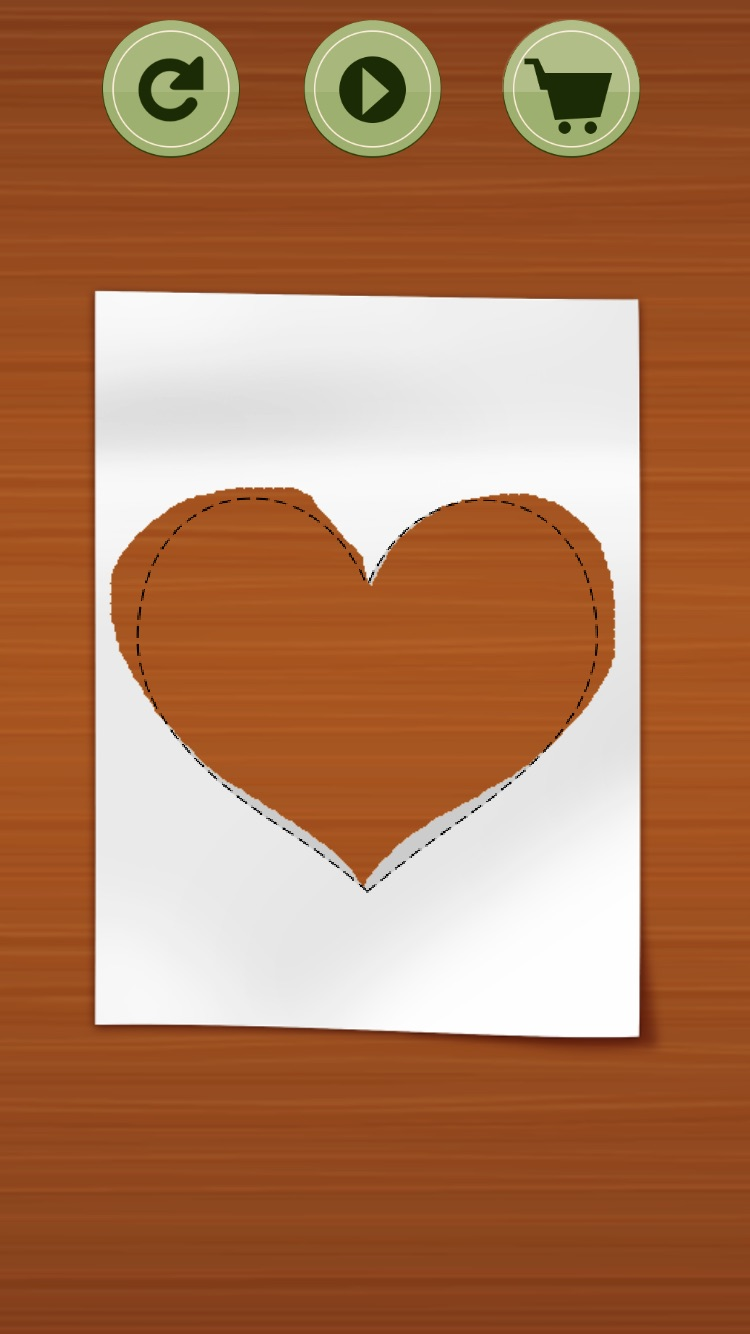
\includegraphics[width=0.25\textwidth]{Images/paperCutCraftReveal}
                    \captionsetup{{margin = 0.2cm}}
                    \caption{This is actually the opposite of what is required. The application decides which part of the paper disappears, the user will not know until after the cut is made.}
                    \label{fig:paperCutCraftReveal}
                \end{wrapfigure}
                
                The shopping basket icon actually refers to the link back to the main selection screen, however this is not clear as the shopping cart implies a section that is purchase only. 
                
                The variety of shapes available to cut is not particularly entertaining. It appears the shape of a cat is the most complex template on the application.
                
                \paragraph{Lessons Learned:}
                
                It is important to have an engaging application. The levels in my application should have variety and complexity and inspire the user. It should be clear how a user ends a level and returns to the home screen.
                
                \subsubsection{Topetope}
                 
                \paragraph{Type:} iPhone application \cite{TopeTope}
                \paragraph{Description:}
                Topetope (``TOPETOPE - cut the square") is an iPhone application that is advertised as a game where the user can cut a square piece of paper, along with cutting challenges that may come with time limits. The application did not appear to be working when tested multiple times with every effort made to troubleshoot it. Most of the application appeared to be inaccessible. 
                
                \paragraph{Strengths:}
                When the application does work (the initial screen shown in \textbf{Figure~\ref{fig:topeReality}} was somewhat functional), the cut of the paper is seamless. The user can drag their finger from one corner to another and the paper is cut along the line and one section falls off via an animation.
                
                \begin{figure}[!ht]
                        \begin{minipage}{0.45\textwidth}
                            \centering
                            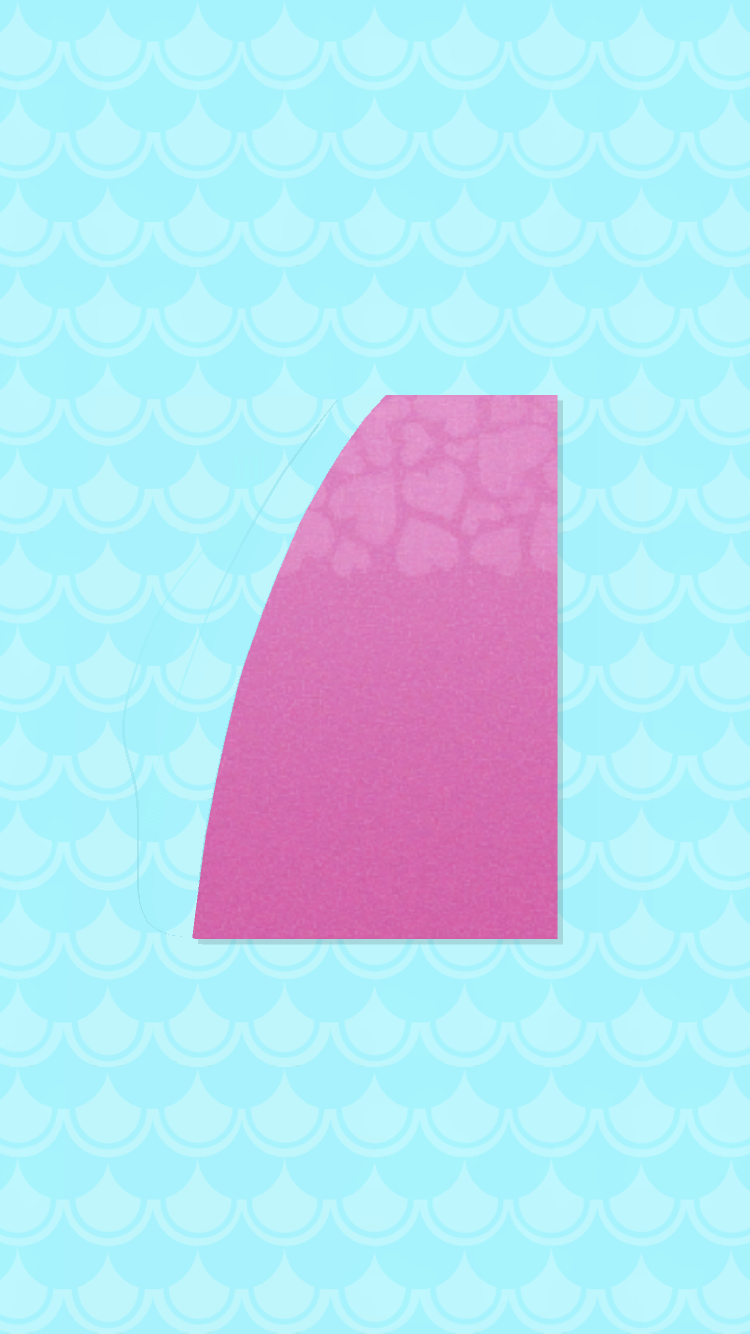
\includegraphics[width=0.6\linewidth]{Images/topeReality}
                            \captionsetup{margin = 0.5cm}
                            \caption{The initial (and only accessible) screen for the app Topetope. The user can use their finger to cut the piece of paper. The application responds approximately half the time.}
                            \label{fig:topeReality}
                        \end{minipage}
                        \begin{minipage}{0.48\textwidth}
                            \centering
                            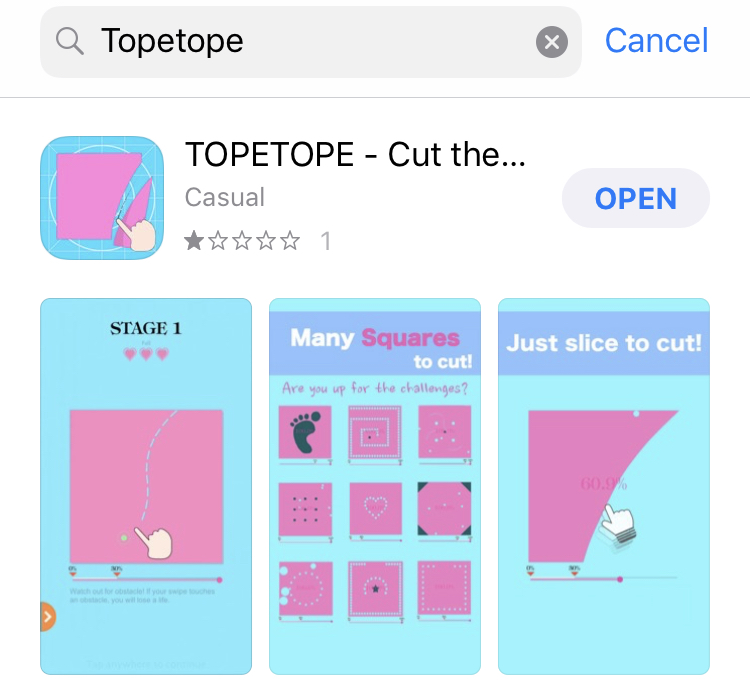
\includegraphics[width=0.85\linewidth]{Images/topeAdvertising}
                            \captionsetup{margin = 0.5cm}
                            \caption{The description for Topetope on the iPhone App Store.}
                            \label{fig:topeAdvertising}
                        \end{minipage}
                    \end{figure}
                    

                \paragraph{Weaknesses:}
                The application is extremely different to the advertised app as seen in figure \textbf{Figure~\ref{fig:topeAdvertising}}. In reality the user is only able to access one screen. With the level that can be accessed, it is unclear what the goal is.
                
                There is no home screen option, navigation available or the presence of tutorial page or directions. The cutting of the paper with the users fingers only works approximately half the time.
                
                The glitching and lack of response from the app is very frustrating.
                
                
                There is no clear meaning of the word ``topetope". May be translated from Spanish meaning the top or stop, however any translation of it does not particularly make sense in context. 
                
                 Topetope also lacked consistency as its description was different to the application.

                \paragraph{Lessons Learned:}
                In contrast to Topetope, the application I create should have a clear and obvious goal. A tutorial may be necessary as this would have been useful in this case. My application should be thoroughly tested at each stage and needs to reliably work throughout. This is especially important due to the relaxing mindfulness component of my application. Another aspect to consider is which side of the paper will disappear after it is cut. I need to make this decision clear if I am making it for the user, or allow the user to choose for themselves. 


       \subsection{Lessons Learned from Similar Applications}
       
            \paragraph{}
            Searching for web applications as well as iPhone apps turned out to be a useful path as Paper Snowflake Maker was the only application where the cutting action worked reliably.
            
            All of the iPhone applications I tested had inconsistencies with their main functionality of cutting shapes out of the segments / virtual paper. However the web application Paper Snowflake Maker did not have such an inconsistency. The expected cut is created from the shape drawn when the cut is finalised and when the unfolded virtual paper is revealed. The application I create should be consistent, reliable and the main feature of cutting should be easy to use.  
            
            Many of the examples had features which either did not fully carry out the expected function or provided no response when interacted with. I will place importance on making all available features work well and to the intended purpose, rather than implementing a large quantity of features. 
            
            None of the iPhone applications I looked at had a cut action that was consistent and worked reliably. All had some sort of glitch to do with the cut. The applications with a larger work space has ease of use. 
            
            A few of the applications had buttons with ambiguous intended functionality, where the same button actually changed functionality depending on the screen. If I choose to use icons, the action of the button should be apparent. Consistency with the format of the buttons can also be important e.g. the buttons I create could all have a similar style for navigation. Some of the applications above lacked this consistency with their buttons. 
            
            Many of the applications reviewed had a snowflake / Christmas theme. Although this may be a good marketing tactic, I do not wish to restrict the kirigami to 3 folds (6 segments) and would like to make something diverse that is different to what is already available and not restricted to seasonal use. I also do not want to restrict the age range by using a popular character like Peppa Hippo or creating my own version. However I will try and extract the features that kept a coherent theme in that application.
            
            The size of the virtual paper should be large enough on the screen to allow for ease of interaction. The method which the user interacts with the paper should be simple and where the cut will occur should be clear (for example, clear which part of the paper is cut and an inverted cut should be easy to carry out). Another major flaw with a few of the application was that there is no clear goal or task. I should try to create an application where the goal or task is obvious.


\newpage
\section{Prototype}

    \subsection{Target User}
    
            \paragraph{}
            Similarly to origami and kirigami, my application will have no specific target audience. However, an interest in Japanese culture and paper crafts is expected. As the name I have chosen for the app are Japanese words, this target audience will be drawn to it. I have highlighted a few key groups below. 
            
            \paragraph{Children}
            This application is especially beneficial for children. Visualising how the shapes they are creating will unfold, or how the shapes already created derive from a single folded component, will allow them to practice mathematical skills, geometry, fractions and spacial awareness.
            
            In addition, the application can be used to enhance children's creativity and encourage them to try the creations they made on the application in real life. 
            
            \paragraph{Young Professionals and Adults}
            An advantage of the application is that you can spend as little or as much time as you like interacting with it. This can be ideal for commuting where the application's mindfulness aspect can be utilised while on public transport.

            \paragraph{Elderly}
            The elderly can use the application to visualise and could help them practice fine touch and co-ordination. It will prove stimulating to consider 2D shapes in an interactive way. 
            \clearpage
            
            \subsection{First Generation}
                    
                \paragraph{}
                Initially I created sketches of views for the first generation prototype and used the application ``POP - Prototyping on Paper" \cite{POP} to make the sketches interactive. The application allows you to create links from one page to another for specified areas of the sketch. This allows the user to essentially click on buttons to link them to the next screen, as seen in \textbf{Figure~\ref{fig:popLinks}}. I linked the screens shown in  \textbf{Figure~\ref{fig:popMultiple}} via the relevant buttons so the user can walk through the application as if they were using it.
                
                I used this POP application to test my prototype out on potential users. The feedback was mainly positive, especially as wire frames are not commonly interactive which allowed for a more authentic user experience. The diagrams were clear so it was easy for the user to understand the concept of the app even with just links to the different pages as the interactivity.
                Link to my specific POP project: https://marvelapp.com/c49jjie
                
                \begin{figure}[!ht]
                        \begin{minipage}{0.45\textwidth}
                            \centering 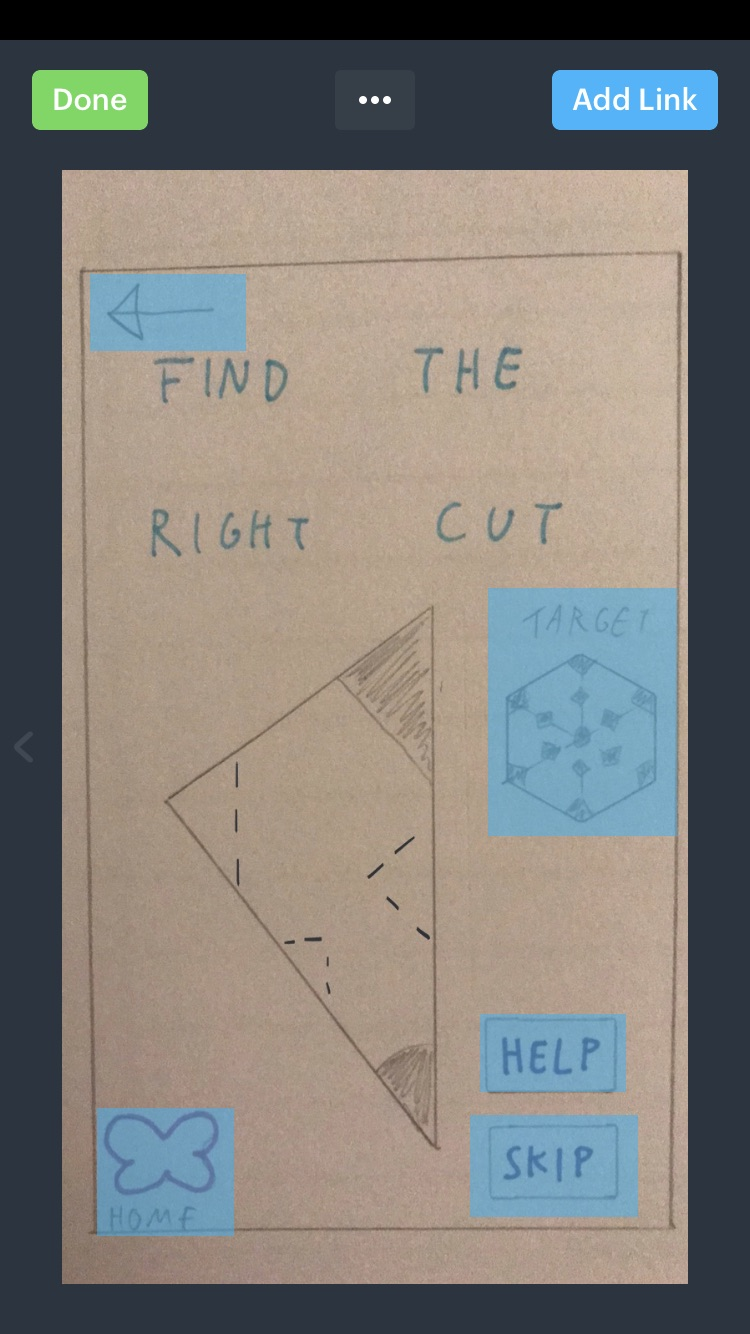
\includegraphics[width=0.7\linewidth]{Images/popLinks}
                            \caption{This figure illustrates how links are made in the POP application to other pages of the app.}
                            \label{fig:popLinks}
                        \end{minipage}\hfill
                        \begin{minipage}{0.45\textwidth}
                            \centering
                            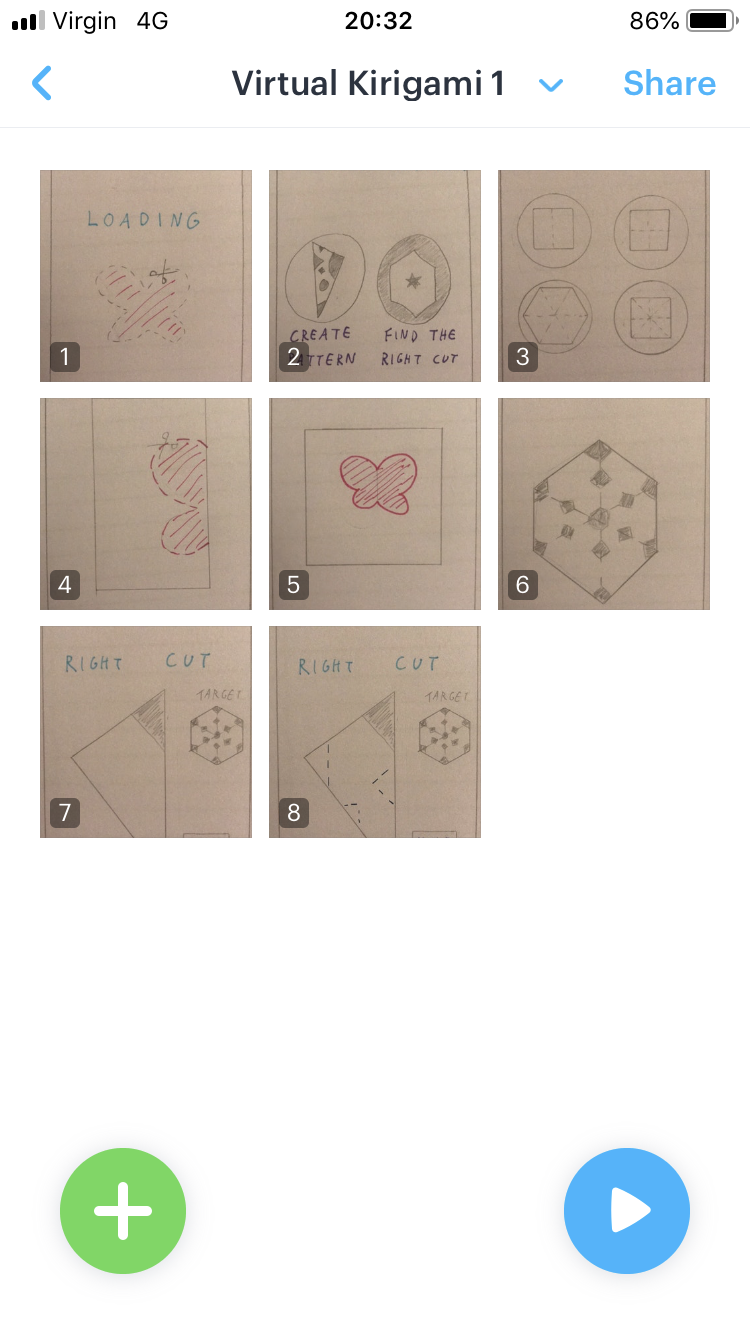
\includegraphics[width=0.7\linewidth]{Images/popMultiple}
                            \caption{All the screens I created for my first generation prototype and linked together in the POP application.}
                            \label{fig:popMultiple}
                        \end{minipage}
                    \end{figure}
                    
                The feedback included suggestions such as relevant titles for pages or no titles for some pages. The home button on every page is unnecessary as the app does not have a large number of screens. Undo and clear buttons should be included when creating the cuts. A save or share button could potentially be included for the unfolded pattern.
                 
            
    \subsection{Second Generation}

        After collating the feedback, I translated the sketches to second generation prototypes on balsamic \cite{Balsamiq}. The prototypes are fully described below. 
    
\clearpage
             \begin{figure}
                \begin{minipage}[c]{0.35\textwidth}
                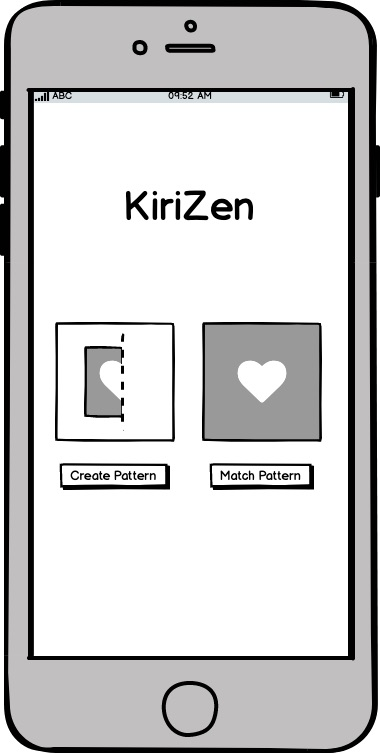
\includegraphics[width=1\textwidth]{Images/Prototype/prototypeHomeScreen}
                \end{minipage}\hfill
                \begin{minipage}[c]{0.65\textwidth}
                \captionsetup{font={normalsize}, margin = 1cm}
                \caption{The home screen will display the graphics for the two parts of the application - ``Create Pattern" and ``Match Pattern". The images used for the buttons will display a pattern being created and a target image respectively. Clicking on the ``Create Pattern" button will link the user to \textbf{Figure~\ref{fig:chooseFold}}, and clicking on ``Match Pattern" will take the user to \textbf{Figure~\ref{fig:target}}.}
                \label{fig:homeScreen}
                \end{minipage}
            \end{figure}
            \begin{figure}
                \begin{minipage}[c]{0.65\textwidth}
                \captionsetup{font={normalsize}, margin = 1cm}
                \caption{This figure is where the user will be able to choose how they want their virtual piece of paper folded. The images for each button will show the crease lines for the virtual piece of paper if it were folded in half, quarters, sixths and eights with straight edges. The user will press one of these buttons which will link them to the corresponding version of the screen shown in \textbf{Figure~\ref{fig:createPattern}}. The left arrow will return the user to the previous screen (\textbf{Figure~\ref{fig:homeScreen}}).}
                \label{fig:chooseFold}
                \end{minipage}\hfill
                \begin{minipage}[c]{0.35\textwidth}
                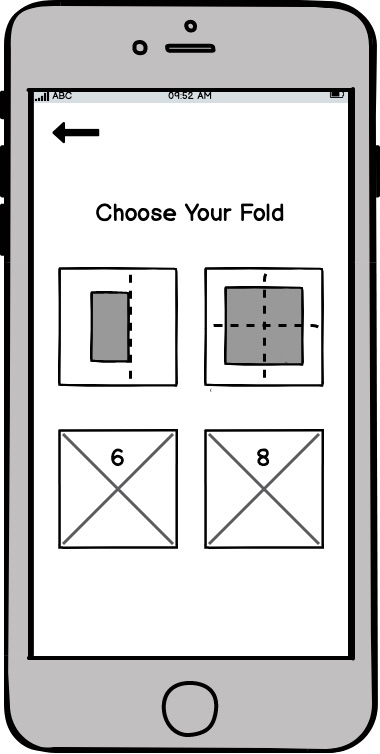
\includegraphics[width=1\textwidth]{Images/Prototype/prototypeChooseFold}
                \end{minipage}
            \end{figure}
            
            \begin{figure}
                \begin{minipage}[c]{0.35\textwidth}
                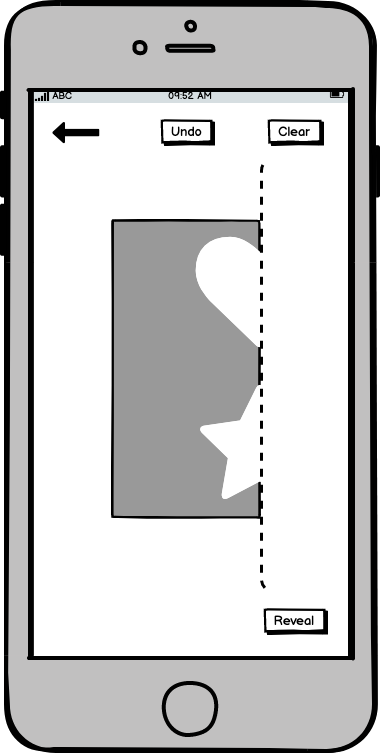
\includegraphics[width=1\textwidth]{Images/Prototype/prototypeCreatePattern}
                \end{minipage}\hfill
                \begin{minipage}[c]{0.65\textwidth}
                \captionsetup{font={normalsize}, margin = 1cm}
                \caption{The shape of the folded segment and dashed lines indicating creases will depend on which button was pressed in \textbf{Figure~\ref{fig:chooseFold}}. The screen displayed here is as if the user pressed the fold in half button. On this screen, the user will create the cuts from the virtually folded piece of paper. They will have the option of deleting the last cut with the ``Undo" button, or refreshing the canvas with the ``Clear" button. Pressing the reveal button will take the user to the next screen (\textbf{Figure~\ref{fig:reveal}}). The left arrow will return the user to the previous screen (\textbf{Figure~\ref{fig:chooseFold}}) and progress will be reset.}
                \label{fig:createPattern}
                \end{minipage}
            \end{figure}
            
            \begin{figure}
                \begin{minipage}[c]{0.65\textwidth}
                \captionsetup{font={normalsize}, margin = 1cm}
                \caption{The unfolded version of the pattern the user created in the previous screen is displayed on this screen. The revealed image will depend on what button was pressed initially to chose the fold. The left arrow will return the user to the previous screen (\textbf{Figure~\ref{fig:createPattern}}).}
                \label{fig:reveal}
                \end{minipage}\hfill
                \begin{minipage}[c]{0.35\textwidth}
                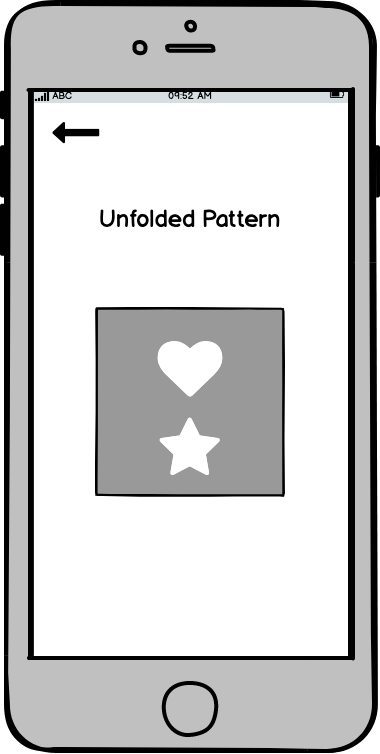
\includegraphics[width=1\textwidth]{Images/Prototype/prototypeReveal}
                \end{minipage}
            \end{figure}
            
           \begin{figure}
                \begin{minipage}[c]{0.35\textwidth}
                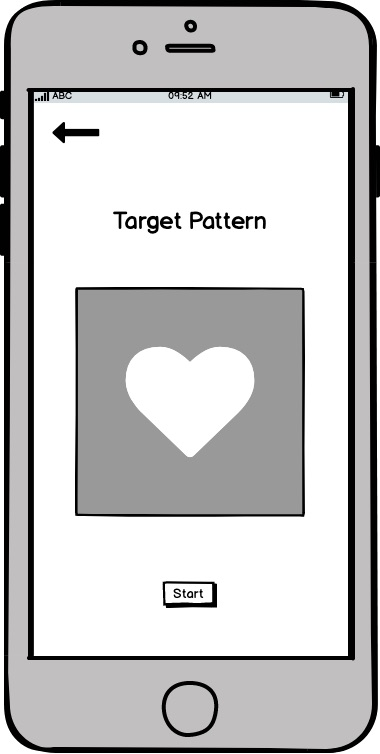
\includegraphics[width=1\textwidth]{Images/Prototype/prototypeTarget}
                \end{minipage}\hfill
                \begin{minipage}[c]{0.65\textwidth}
                \captionsetup{font={normalsize}, margin = 1cm}
                \caption{A random target pattern will be displayed for the user. They can press the start button to link them to the next screen (\textbf{Figure~\ref{fig:matchPatternCreate}}) to start cutting. The left arrow will return the user to the previous screen (\textbf{Figure~\ref{fig:homeScreen}}).}
                \label{fig:target}
                \end{minipage}
            \end{figure}
                           
           \begin{figure}
                \begin{minipage}[c]{0.65\textwidth}
                \captionsetup{font={normalsize}, margin = 1cm}
                \caption{As before in \textbf{Figure~\ref{fig:createPattern}}, the folded segment and dashed lines indicating creases will depend on the target pattern shown in the previous page. The screen displayed here is as if the target image was created from the virtual piece of paper being folded in half. The user has the option of pressing the help button (explained in \textbf{Figure~\ref{fig:matchPatternCreateHelp}}) or the target button which will show the user the target image again without resetting their progress. The user again will have the option of deleting the last cut with the ``Undo" button, or refreshing the canvas with the ``Clear" button. Pressing the reveal button will take the user to the next screen (\textbf{Figure~\ref{fig:reveal}}). 
                The left arrow will return the user to the previous screen (\textbf{Figure~\ref{fig:target}}) and progress will be reset.}
                \label{fig:matchPatternCreate}
                \end{minipage}\hfill
                \begin{minipage}[c]{0.35\textwidth}
                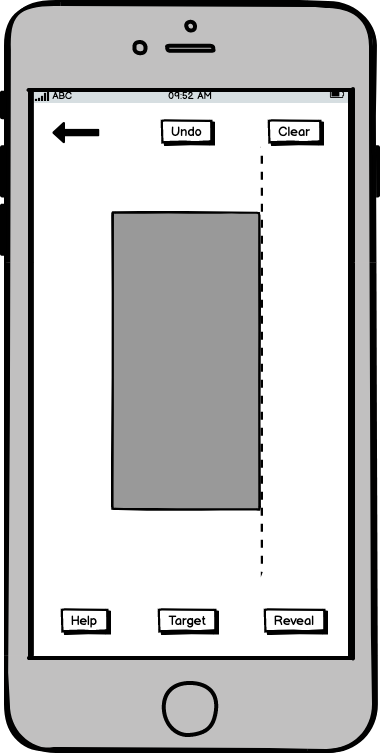
\includegraphics[width=1\textwidth]{Images/Prototype/prototypeMatchPatternCreate}
                \end{minipage}
            \end{figure}

            \begin{figure}
                \begin{minipage}[c]{0.35\textwidth}
                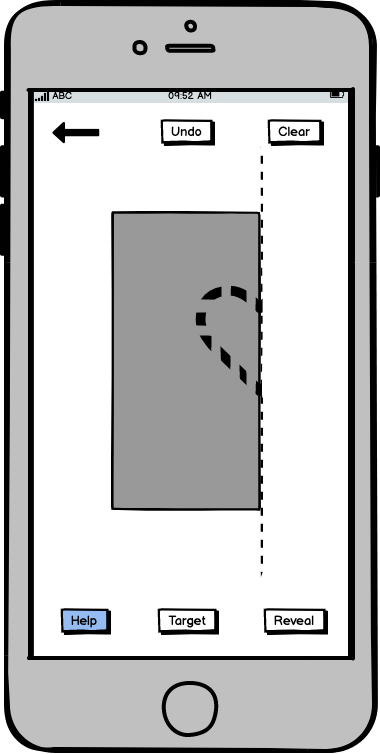
\includegraphics[width=1\textwidth]{Images/Prototype/prototypeMatchPatternCreateHelp}
                \end{minipage}\hfill
                \begin{minipage}[c]{0.65\textwidth}
                \captionsetup{font={normalsize}, margin = 1cm}
                \caption{This is the same screen as \textbf{Figure~\ref{fig:matchPatternCreate}}, but with the help button pressed. This button will show the user where they need to create the cuts. The user will be able to toggle this button on and off.}
                \label{fig:matchPatternCreateHelp}
                \end{minipage}
            \end{figure}
            
            \begin{figure}
                \begin{minipage}[c]{0.65\textwidth}
                \captionsetup{font={normalsize}, margin = 1cm}
                \caption{The unfolded version of the pattern the user created in the previous screen is displayed on this screen. The revealed image will depend on which fold was chosen in the first step. The user will have the option to compare the image they created with the target image they were aiming for. The left arrow will return the user to the previous screen (\textbf{Figure~\ref{fig:matchPatternCreate}}).}
                \label{fig:revealWithOverlay}
                \end{minipage}\hfill
                \begin{minipage}[c]{0.35\textwidth}
                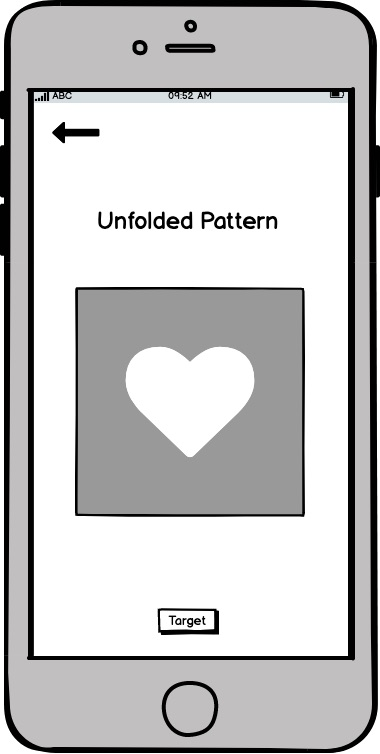
\includegraphics[width=1\textwidth]{Images/Prototype/prototypeRevealWithOverlay}
                \end{minipage}
            \end{figure}
                        \clearpage
            

\newpage
\section{Implementation}

\subsection{Requirements}
    
    \subsubsection{Functional}
    
    \begin{enumerate}
      \item Home Screen
        \begin{enumerate}[label*=\arabic*.]
        \item The application must allow the users to select a ``Create Pattern" button or a ``Match Pattern" button, linking them to the relevant screen.
        \item The application could have an information page linked from the home screen.
        \item The application could have background music controlled via a button on the home page.
      \end{enumerate}
      
       \item Choose Fold
        \begin{enumerate}[label*=\arabic*.]
        \item The application must allow the user to choose whether they want the virtual piece of paper folded into 2, 4, 6 or 8 sections.
      \end{enumerate}
      
      \item Creating cuts
      \begin{enumerate}[label*=\arabic*.]
        \item The application must display the corresponding shape of the folded piece of paper depending on which fold was selected in the previous screen.
        \item The application must indicate which side(s) are folded via the display of a dashed line(s).
        \item The application must only allow the user to tap on screen outside the virtually folded paper to start a cut. 
        \item The application must allow the user to tap on screen to set the corners of a cut.
        \item The application should indicate to the user where the start of their cut.
        \item The application should allow the user to complete their cut by tapping near the start of their cut. 
        \item The application must display the reveal screen upon selection of a corresponding button.  
         \item The application should have an undo button.
          \item The application should have a clear button.
        \item The application should have an instructions page available on the cut screens. 
      \end{enumerate}
      
      \item Match Pattern
        \begin{enumerate}[label*=\arabic*.]
        \item The application must display the target image to the user.
        \item The application must allow the user to attempt to recreate the cut free of help. 
        \item The application must allow the user to see the target image again from this page. 
        \item The application should allow the user to select an overlay option for help.
      \end{enumerate}

       \item Reveal
          \begin{enumerate}[label*=\arabic*.]
            \item The application must show the user an unfolded version of their cuts from the corresponding folded virtual piece of paper. 
            \item The application must allow the user to compare their pattern with the target pattern when selected via the match pattern section.
            \item The application could have a pinch zoom feature for the virtual unfolded creation.
            \item The application could allow the user to save their virtual unfolded creation to their camera roll.
            \item The application could have a share button exporting the image to other applications. 
          \end{enumerate}
        \end{enumerate}

    
   \subsubsection{ Non-Functional}
    
    \begin{enumerate}
        \item Performance
            \begin{enumerate}[label*=\arabic*.]
            \item The application should respond to the users touch within 0.5 seconds while making the cuts.
            \item The application should take no longer than 5 seconds to load up after it has been downloaded onto the iPhone.
            \end{enumerate}
            
        \item Usability
            \begin{enumerate}[label*=\arabic*.]
            \item The average user should be familiar with the application after 5 minutes of use. 
            \item The average user should be able to understand the flow/navigation of the application easily.
            \end{enumerate}
            
        \item Availability
            \begin{enumerate}[label*=\arabic*.]
            \item The application must be available on iPhone 7 and 8.
            \end{enumerate}
            
        \item Reliability
            \begin{enumerate}[label*=\arabic*.]
            \item The application must perform as specified.
            \item The application shall be available 99\% of the time 24/7.
            \end{enumerate}
         
    \end{enumerate}
    \clearpage
    
    \subsection{Overview}

    \begin{wrapfigure}{r}{0.35\textwidth}
                        \centering
                        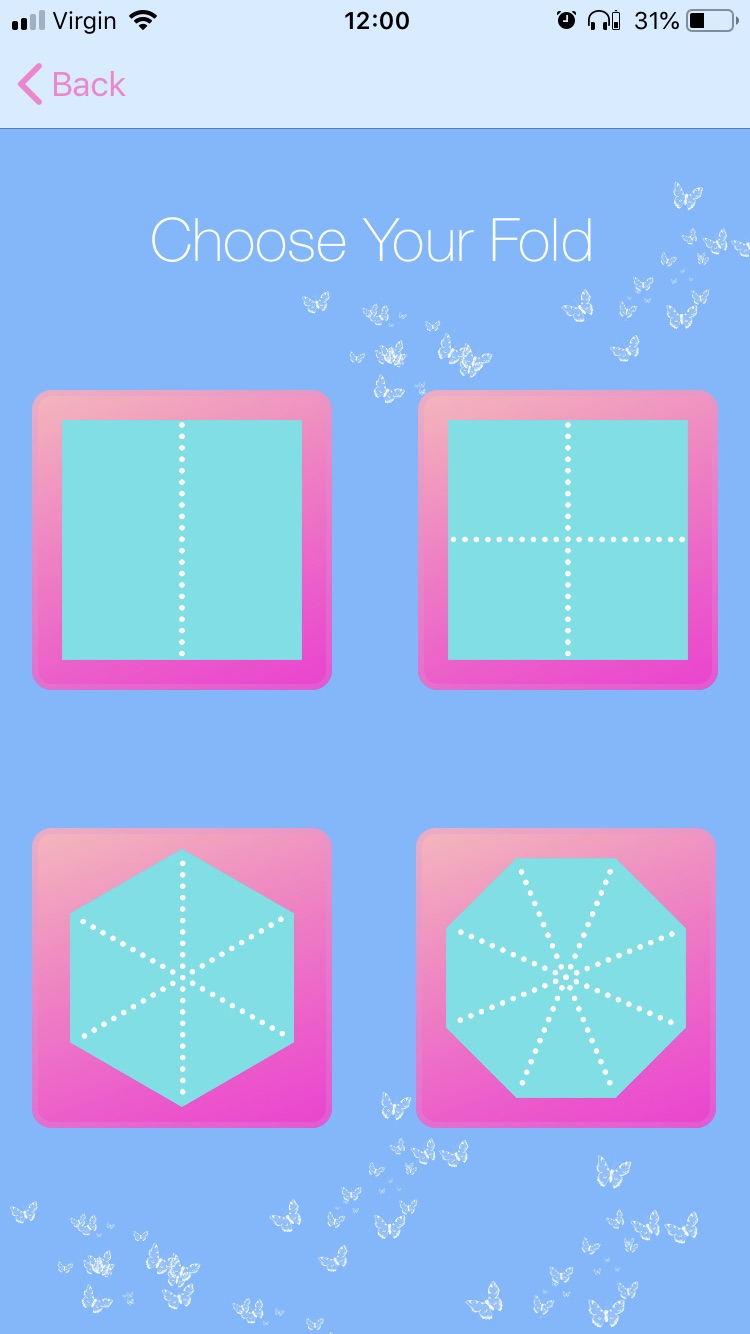
\includegraphics[width=0.3\textwidth]{KiriZen/chooseFold}
                        \caption{The display associated with ``ChooseFoldVC". The buttons represent the folds the piece of paper will be virtually folded into.}
                        \label{fig:kiriZen-chooseFold}
                    \end{wrapfigure}
    

    \paragraph{}
    I used the storyboard in Xcode to lay out the general overview of the application. This visualisation was handy when creating segues between the classes as I could clearly see which classes were interacting. The Navigation Controller was used so the user will be familiar with the flow of the app quickly. The Navigation Controller is the bar at the top of \textbf{Figure~\ref{fig:kiriZen-chooseFold}} and is present on all screens.
    
        \subsection{Choose Fold}

        \paragraph{}
            In the storyboard for ``ChooseFoldVC", I assigned a tag for each button related to how many segments the folds split the paper into. For the rest of this section I will refer to this value as the foldValue. Segues are transitions between view controllers which can be labelled in the storyboard. I added segues from each button to the next view controller.
                    
            In the class ``ChooseFoldVC", when one of the buttons in \textbf{Figure~\ref{fig:kiriZen-chooseFold}} is pressed, I assign a variable to the foldValue of the tag. This information is then carried to the next view controller overriding the ``prepare" function. This function transfers the foldValue information from ``ChooseFoldVC" to ``CreatePatternVC", by assigning the information from a variable in ``ChooseFoldVC" to a variable in ``CreatePatternVC".
                    
            The use of tags and segues is important as the button pressed in ``ChooseFoldVC" (and equivalent values for the target pattern produced later on in the Match Pattern section) as it determines the shapes drawn representing the virtual piece of paper of the upcoming view controllers. It also determines the number of copies of the created pattern, and how they will be transformed and revealed.
            
                
            \subsection{Create Pattern and Canvas}
                \paragraph{}
                ``CreatePatternVC" is the view controller for the screen where cuts are created on the virtual folded piece of paper. This class displays the buttons in stack views. I grouped the buttons according to functionality with undo and clear next to each other, and instructions/ information buttons are always blue in this application to keep consistency. 
                
                ``CreatePatternVC" creates a UIView called canvas where the functions associated with cutting can occur.
                    
                 \paragraph{Cutting Shapes}
                 The foldValue determines which shape of what dimensions will be created in the draw function. When this function is called, the shape is drawn and the parameters for the dashed lines are set and the function to draw the dashed line is called. The lines indicate to the user the sides of the segment that were folded and can be seen in \textbf{Figure~\ref{fig:kiriZen-createPattern}}.
                 When cuts are made from the shape, I wanted the dashed lines to appear intact so the user does not have to recall were the folds are. I decided to make the majority of shapes created of the type CAShapeLayer. This was to make it simple to layer the shapes in the order I desired. When cuts were made from the virtual paper, I could bring the dashed line shape to the front of the view easily. This effect is illustrated in \textbf{Figure~\ref{fig:kiriZen-createPattern}} where some shapes have already been cut.
                 
                 The user can create the cuts by tapping on the screen. I decided that the user must be able to cut from the edge of the paper. This is to make the transition to real life easier if the user wanted to try out their creations. To cut with scissors, you must start of the edge of the paper, not in the middle as this is difficult to do with multiple folds of paper. I also decided not to remove the smaller pieces of paper as those can make for interesting patterns, and I do not wish to make the decision for the user which pieces they would like to keep, and which they would like to discard.
                 
                 \begin{table}[h!]
                      \begin{center}
                      \caption{Data structures associated with didTap(), the main function to cut shapes out of the virtual paper.}
                      \label{tab:table1}
                        \begin{tabular}{|l|l|p{8cm}|}\hline
                          \textbf{Varibale Name} & \textbf{Type} & \textbf{Comments}\\\hline
                          tapPoint & CGPoint \centering & Contains the co-ordinates of the tap.\\\hline
                          initialTap & CGPoint & Contains the co-ordinates of the initial tap.\\\hline
                          tapCount & Int & Incremented with each tap. It helps to determine the progression of the shape being created.\\\hline
                          shapesArray & [CAShapeLayer] & Contains the shapes that have been created.\\\hline
                          pathArray & [CGPoints] & Contains points for the corners of the shape being created.\\\hline
                          circleArray & [CAShapeLayer] & Contains all the circles that are created that represent the corners of the shape.\\\hline
                          lineArray & [CAShapeLayer] & Contains the dotted lines representing the edges of the shape.\\\hline
                         
                        \end{tabular}
                      \end{center}
                    \end{table}
                    
                 To implement the cutting function, I used a number of data structures to hold information. These data structures are described in \textbf{Table~\ref{tab:table1}}. The arrays which hold the CAShapeLayers are for the purpose of removing the shapes when necessary (through the user action of clear and undo, or removing the circles and lines once a user finishes a cut and the cut shape is created. It is important to note that adding to an array in swift (.append) is of complexity O(1) \cite{O1}.
                 
                 I wrote a method didTap() which takes in a UITapGestureRecognizer. The UITapGestureRecognizer contains information about the tap. I compared the colour of the pixels at the location of the tap with the colour of the background. I did this with the methods getPixelColorAt() and comparePixels() which take in the location of the tap and the array of RGB colours of the tap location respectively. The comparePixels() method returns true if the colour is within a given range. This controls for any minor image alterations for the match pattern portion of the app. The overlay image displayed can be slightly distorted in colour as I created the images by taking screenshots of cuts I had made in an earlier version of the application. This distortion is unable to be seen by the naked eye, however it is picked up when analysing the pixel colour. 
                 
                 
                  \begin{wrapfigure}{r}{0.4\textwidth}
                        \centering
                        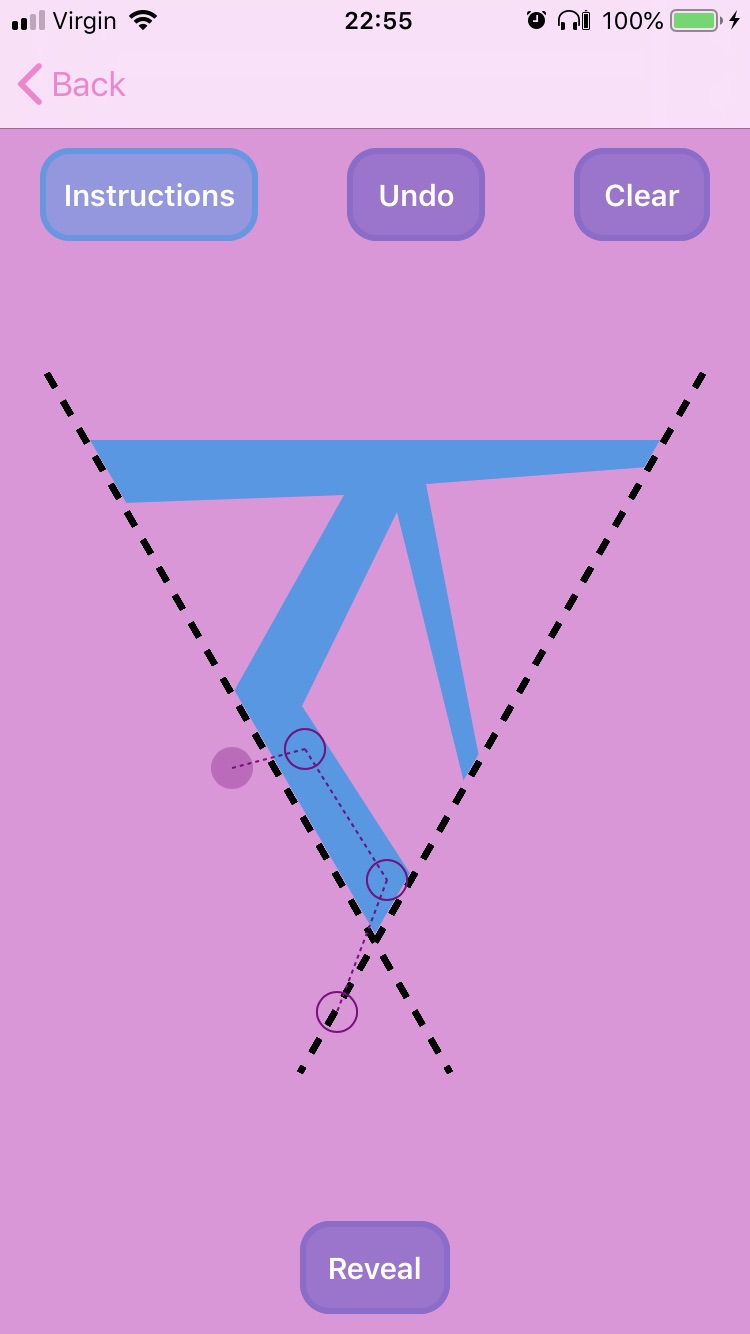
\includegraphics[width=0.35\textwidth]{KiriZen/createPattern}
                        \caption{The user has created three shapes and is partway through making the fourth. The dark purple circle represents the start of the shape they will cut. The clear circles represent the corners of the cuts with the dotted lines representing the edges of the cut.}
                        \label{fig:kiriZen-createPattern}
                    \end{wrapfigure}
                    
                 If the user has tapped outside the virtual paper for their initial tap, a purple circle is displayed to indicate the start point. The circle is displayed and added to the circleArray. The initial tap is recorded, the tap counter is incremented and the co-ordinates added to the pathArray. 
                 
                 As the tapCount is now 1, the first ``if" statement is skipped and there is a check to see if the current tap is within a 20 unit radius (the same size as the circles that are displayed after a tap) of the initial tap. 
                 
                 If it is not, a dotted line is created from the last point to the current point, and added to the lineArray. A clear circle displayed at the current point (to differentiate from the initial tap) and added to the circle array. The current tap co-ordinate is added to the pathArray, and finally the the tap count is incremented. This is repeated as taps occur until the current tap is within a 20 unit radius of the initial tap. In this case, the shape is created. To do this, the pathArray is looped through and a UIBezierPath is created out of the co-ordinates which form the shape that is filled with the background colour. The shape is added to the shapeArray. The circleArray, pathArray, lineArray and tapCount are all reset and the dashedLine() function is called to bring the dashedLine to the front. 

                %Create flow chart of above
            
             \paragraph{Undo and Clear}
              I expanded the functionality of the undo button as I observed that the users were reaching for it when part-way through cutting a shape to edit their last point. 
              When the undo button is pressed, if there are partly constructed shapes, the last circles will be removed from view and then from the circleArray. The last line will also be removed from view and that line removed from the line array if the circle is not the inital point. An ``if" statement checks to see if the arrays are empty before removing anything. If only fully constructed shapes are present the last shape will be removed from the view and from the shape array. The tapCount is also decremented. 
              
              The clear button will reset all the arrays and counters (shapeArray, circleArray, pathArray, lineArray and tapCount).
    

    \subsubsection{Reveal}
            \paragraph{}
            When the reveal button is pressed on the create screen, ``CreatePatternVC" handles the segue to ``RevealVC", transferring the foldValue, and takes a screenshot passing this image through to ``RevealVC". ``RevealVC" makes copies of this screenshot depending on how many segments the pattern created will unfold to. Each copy is transformed with appropriate parameters to create the unfolded image.  
            
            \begin{wrapfigure}{r}{0.25\textwidth}
                        \centering
                        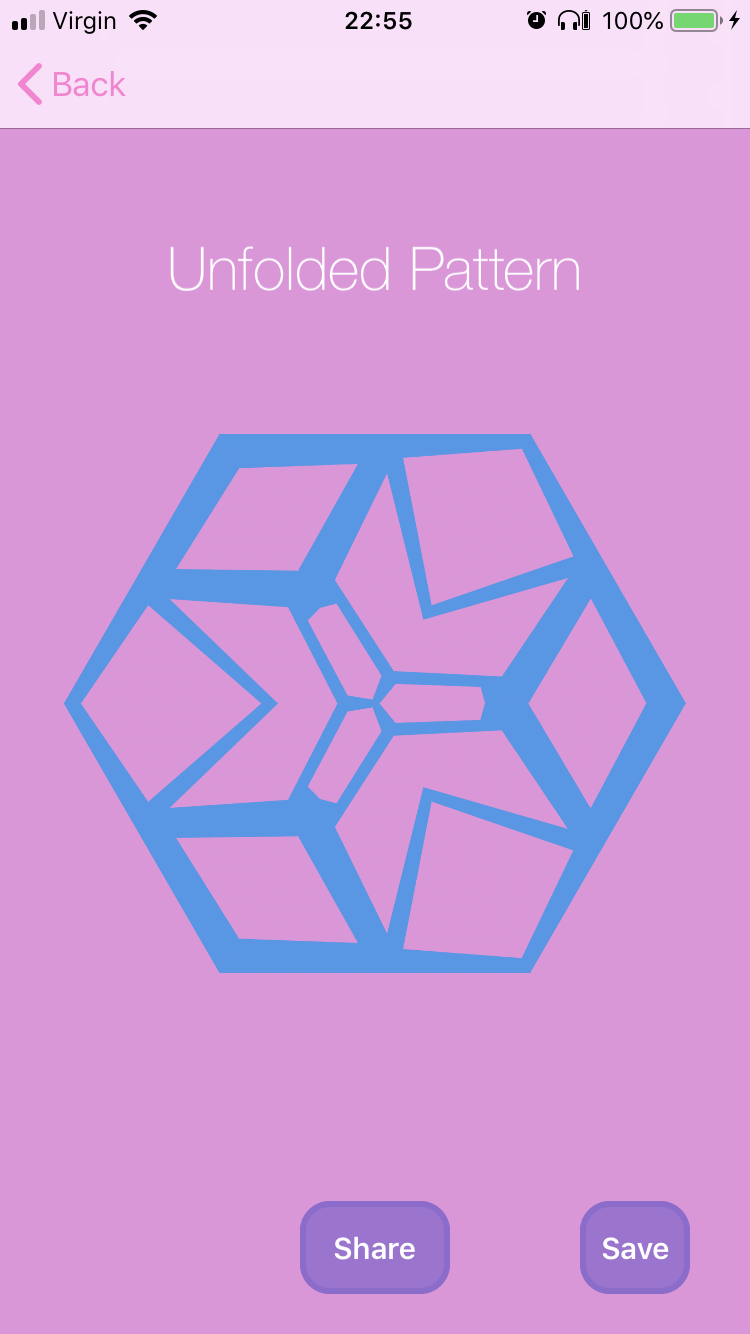
\includegraphics[width=0.25\textwidth]{KiriZen/createUnfoldedPattern}
                        \caption{This pattern created from the cuts made by the user in \textbf{Figure~\ref{fig:kiriZen-createPattern}}. The foldValue here is 6.}
                        \label{fig:kiriZen-createUnfoldedPattern}
                    \end{wrapfigure}
            
            For foldValues of 2 and 4, the images are cropped, copied, and placed in a UIImageView where they are transformed. The images are then added to the subview. 
            
            If the foldValue is 2, the copies of the image of the created pattern are cropped, the image reflected in the horizontal axis, and then it is translated to be opposite the unflipped segment. 
            
            For a foldValue of 4, the copies are cropped, one copy is reflected in the x-axis, another the y-axis and the other one, in both axis. They are translated to their corresponding quadrant. 
                    
            The foldValues of 6 and 8 were much harder to display as images can only be cropped with a rectangle. The solution is to add a CALayer ``mask" to the image which is essentially creating a layer that makes the images underneath invisible with a polygon shaped hole of set dimensions where you can see the image below.
            
            The relevant number of copies were made for the transformations of foldValues of 6 and 8. The transformation also involved rotations in radians, as well as scaling and translating similar to before.
                    
            As there were so many copies of the segments that needed displaying in some cases, a challenge in this class was compressing all the code to the necessary steps. I created one function for transformations that was extremely helpful when refactoring my code as this method was called for almost every copy of the pattern. 
            

    \subsection{Match Pattern}
            \paragraph{}
            This section of the application is adding an additional challenge of asking the user to try and mimic the target image presented. ``Match Pattern" displays a random target pattern to the user. Two random numbers are generated, one representing the foldValue, the other the version of the target pattern for this particular foldValue (there are 5 versions for each foldValue, 20 targets in total). Segues are also used throughout this portion of the app to carry over the foldvalue and version number. An example of the target patterns are seen in \textbf{Figure~\ref{fig:kiriZen-simpleTarget}} and \textbf{Figure~\ref{fig:kiriZen-complexTarget}}. The users can press the start button when they are ready to recreate the pattern.
                    
        \subsubsection{Match Create}
            \paragraph{}
            For the rest of the match pattern section, I inherited from the relevant classes in the create pattern section. This was important as this allowed me to reuse the code without copying it. It was also very useful as this helped features such as the buttons stay consistent as they were displayed in the same location and had same appearance. The shape of the folded segments were also the same. The inheritance helps the user use recognition rather than recall, making the application easier to use. 

            \begin{figure}[!ht]
                        \begin{minipage}{0.45\textwidth}
                            \centering 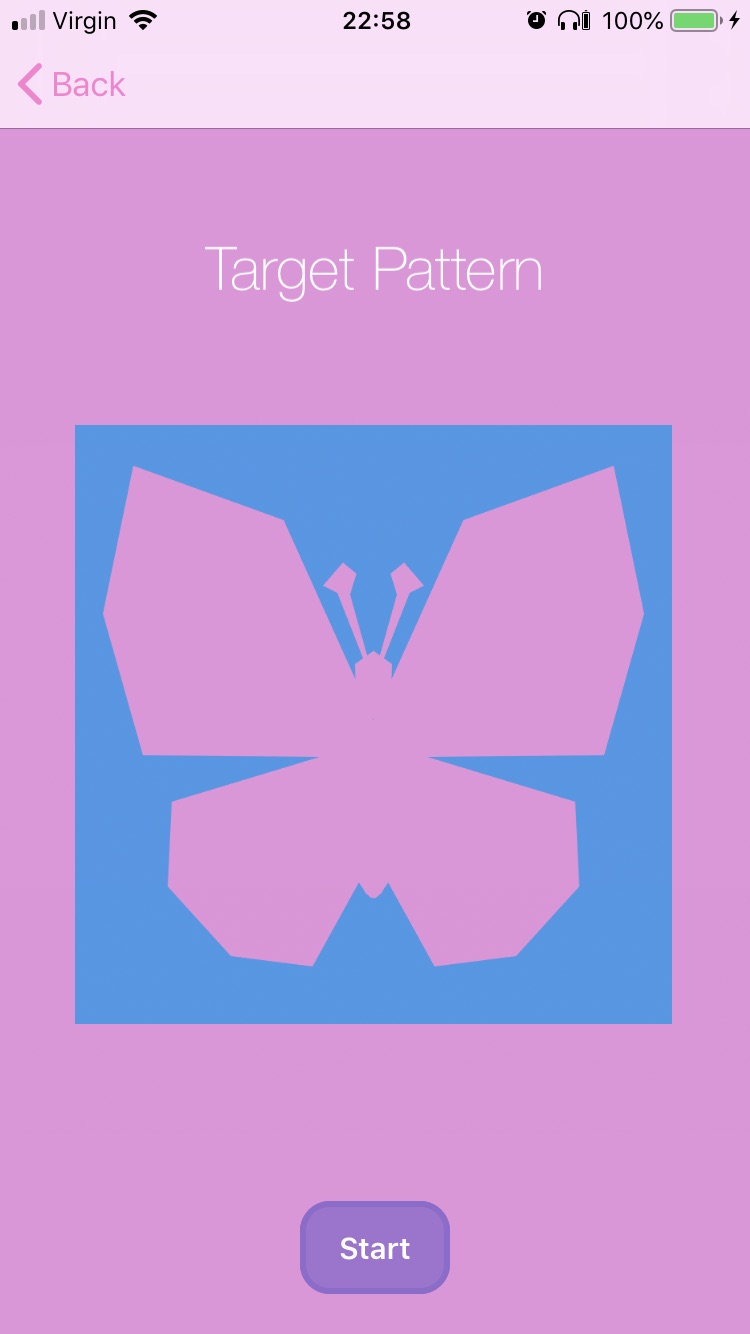
\includegraphics[width=0.7\linewidth]{KiriZen/simpleTarget}
                            \caption{A simple target pattern created by using the create pattern activity in the application. This particular target represents the theme of the application. The foldValue of this pattern is 2.\\}
                            \label{fig:kiriZen-simpleTarget}
                        \end{minipage}\hfill
                        \begin{minipage}{0.45\textwidth}
                            \centering
                            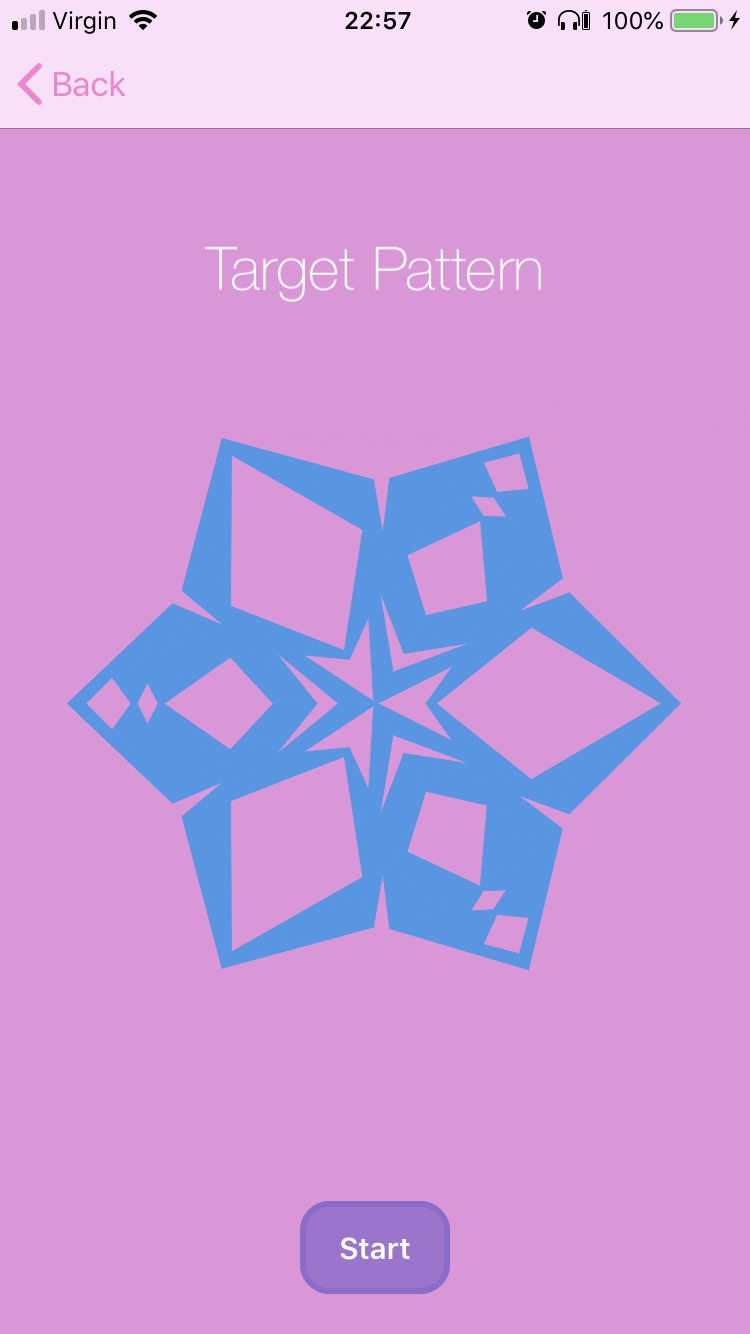
\includegraphics[width=0.7\linewidth]{KiriZen/complexTarget}
                            \caption{A complex target pattern created by using the create pattern activity in the application. The more complex patterns is also aimed to inspire the users to create more complex patterns.  The foldValue of this pattern is 6.}
                            \label{fig:kiriZen-complexTarget}
                        \end{minipage}
                    \end{figure}
                    
                    \begin{wrapfigure}{r}{0.3\textwidth}
                        \centering
                        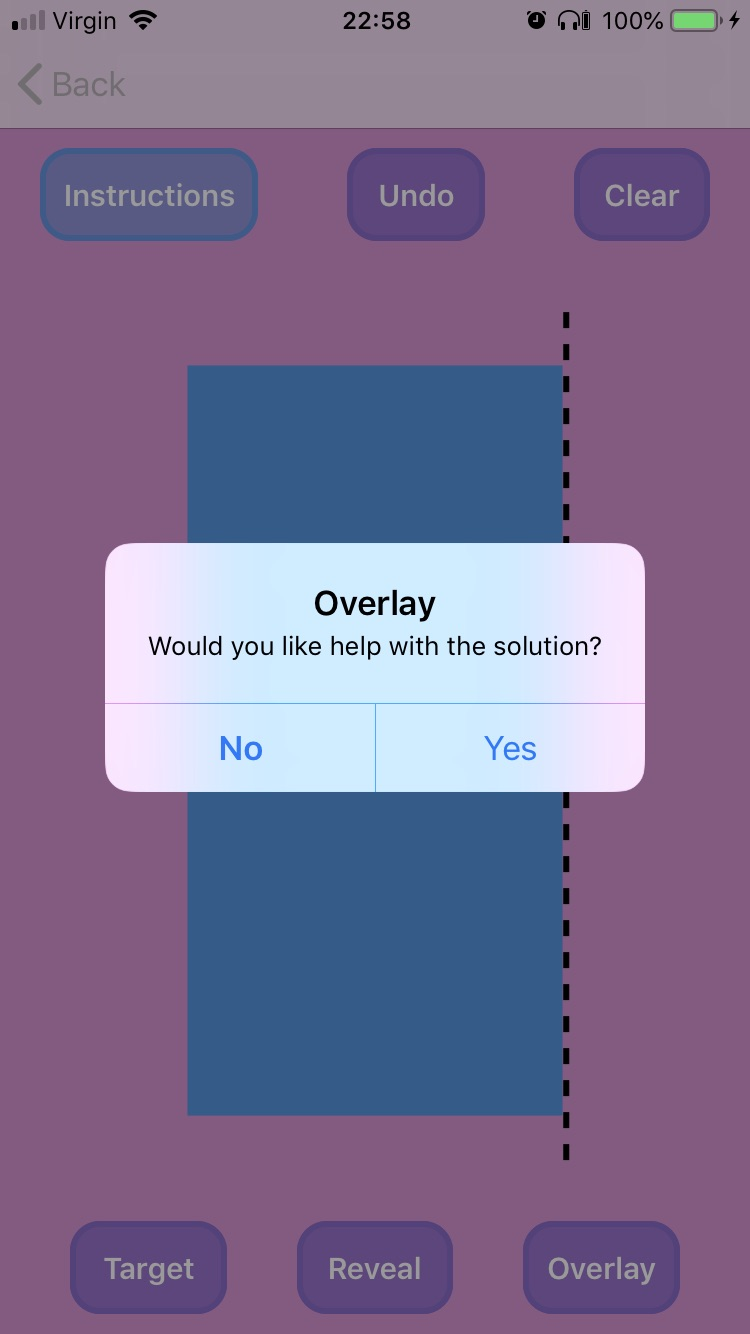
\includegraphics[width=0.25\textwidth]{KiriZen/overlayPopUp.jpeg}
                        \caption{This pop-up is displayed when the user presses the overlay button if they have not accepted the help yet (selected yes).}
                        \label{fig:kiriZen-overlayPopUp}
                    \end{wrapfigure}
                    
                    In addition to the ``CreatePatternVC", a target button and overlay button were also added as seen in \textbf{Figure~\ref{fig:kiriZen-overlayPopUp}} and \textbf{Figure~\ref{fig:kiriZen-matchCreateOverlay}}. When the overlay button is pressed, an alert is created. It warns the users that pressing this button will show them how to create the pattern and is a clue in solving the challenge. An example of the overlay alert is seen in \textbf{Figure~\ref{fig:kiriZen-overlayPopUp}}. The UIAlertController is used which will be a familiar format for the iPhone user. A counter is incremented when the user selects "Yes" for the first time. The overlay button will then toggle between revealing the solution and removing it from the view when pressed. The overlay button is highlighted in blue when the overlay is visible as seen in \textbf{Figure~\ref{fig:kiriZen-matchCreateOverlay}}. The important aspect of overlay image is that it must be aligned precisely with shape of the virtual segment of paper underneath. The image has an alpha value of 0.5 meaning it is halfway between totally transparent (0) and opaque (1.0) so the user can see both their cut, and the cuts they are aiming for. 
                    
                    The target button will display the target image to the user when held down. This is so the user does not have to return to the previous screen to see the target which would reset their progress. There are various events that can occur depending on the users physical interaction with a button on screen shown in \textbf{Table~\ref{tab:table2}}.
                    
                    \begin{table}[h!]
                      \begin{center}
                      \caption{Actions for user interaction}
                      \label{tab:table2}
                        \begin{tabular}{|l|p{8cm}|}\hline
                          \textbf{Action Name} & \textbf{Action Trigger}\\\hline
                            touchDown & The user presses down on the button within its boundaries (occurs before touchUpInside) \\\hline
                            touchUpInside & The user presses down on the button within its boundaries (occurs after touchDown) \\\hline
                            touchCancel & The touch is cancelled (from a system trigger) \\\hline
                            touchDragOutside & The users drags their finger outside the button's boundaries\\\hline
                        \end{tabular}
                      \end{center}
                    \end{table}
                    
                    The target button displays the target image with the ``touchDown" action, and removes the image with ``touchUpInside", ``touchCancel", and ``touchDragOutside". Without this, the target image would be left on the screen if the user performs certain actions or if the system cancels an action. This would allow the user to be able cut shapes on the background screen even with it being blocked by the target image creating a problem similar to that of the the problem seen in \textbf{Figure~\ref{fig:peppaGlitchLine}} (the line is drawn on top of the pop-up in the application). In addition the user may not be able to remove the target image from view. 
                    
                    The overlay button is activated when touchDown or touchDragOutside occurs which will show the alert until ``Yes" is selected. It will subsequently add or remove the overlay from the screen when pressed (depending on if it is already displayed or not).
                    
                    \begin{figure}[!ht]
                        \begin{minipage}{0.45\textwidth}
                            \centering 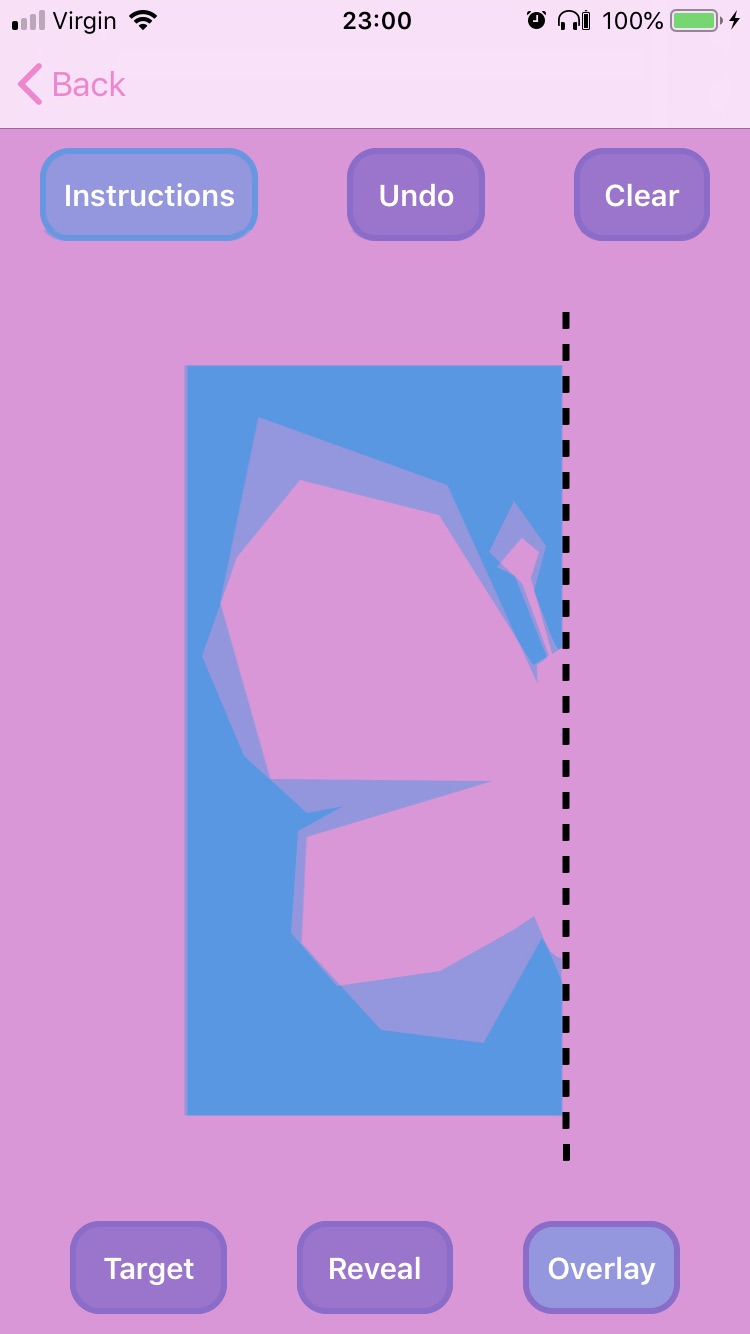
\includegraphics[width=0.7\linewidth]{KiriZen/matchCreateOverlay}
                            \caption{This is what the user will see once the overlay is displayed. They can see an outline of where the shape should be and they will still be able to see the cuts they made underneath.\\}
                            \label{fig:kiriZen-matchCreateOverlay}
                        \end{minipage}\hfill
                        \begin{minipage}{0.45\textwidth}
                            \centering
                            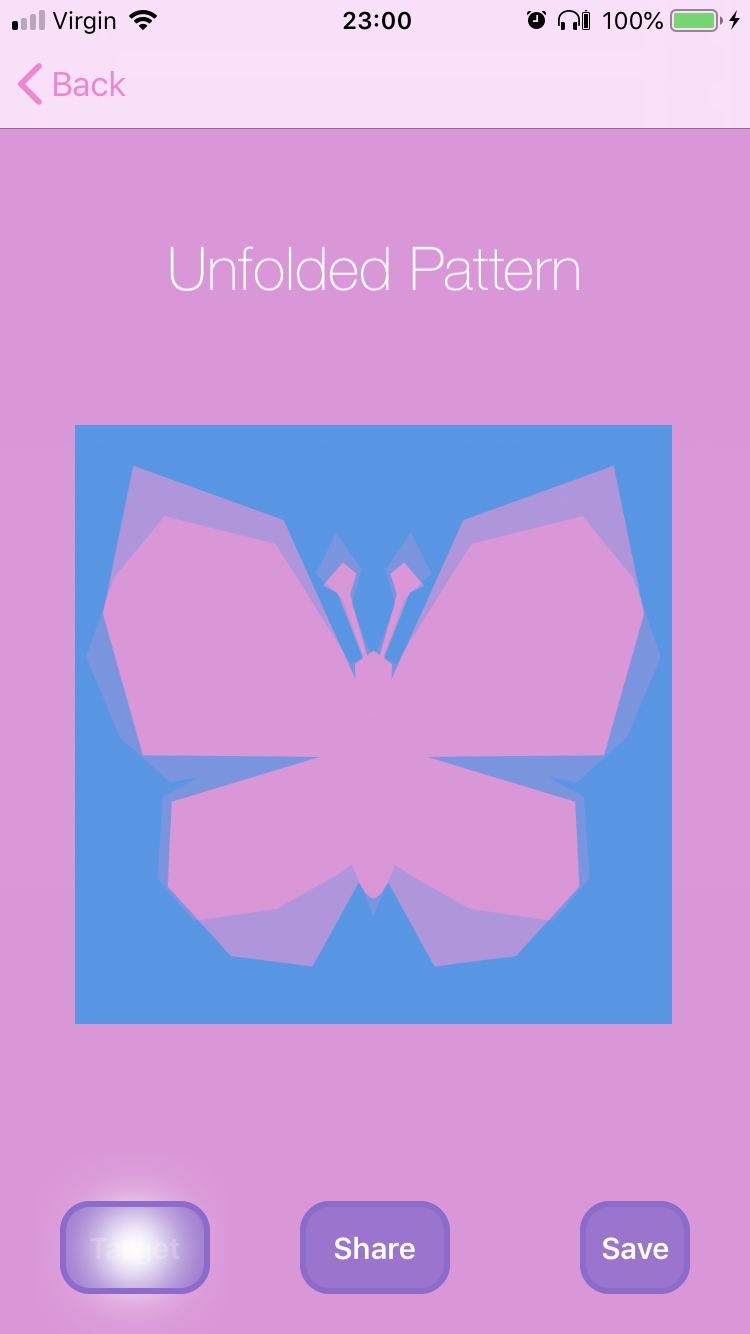
\includegraphics[width=0.7\linewidth]{KiriZen/matchUnfoldedPattern}
                            \caption{This the what the user will see when they hold down the target button on the reveal page. They can see the outline of the shape they were aiming for and can compare it to their creation.}
                            \label{fig:kiriZen-matchUnfoldedPattern}
                        \end{minipage}
                    \end{figure}
            
 \subsubsection{Reveal Match VC}
            \paragraph{}
            ``RevealMatchVC" inherits from ``RevealVC" therefore using the foldValue information passed via segues, it can construct the unfolded image as before in the create pattern section. There is an additional feature on this screen of the target button. When held down, the target is overlayed onto the image which was created to allow the user to compare their creation with the target they were aiming for. The target image has an alpha value of 0.7 allowing the user to see their image underneath as in \textbf{Figure~\ref{fig:kiriZen-matchUnfoldedPattern}}.

\clearpage
\newpage
\section{Human Computer Interaction}
    
    \subsection{Theme}
        
        \paragraph{}
        The name of the app ``KiriZen" is a combination of the words ``kiri" and ``zen". Kiri as previously mentioned, refers to the Japanese word meaning ``to cut". The word zen has connotations of peace and relaxation. These words encompass what I am trying to achieve with the app. I am aiming to make the the users feel relaxed while creating or matching the kirigami patterns.
        
        Upon researching the name, no similar applications, products, or concepts that could potentially lead users elsewhere were found. Therefore if I were to publish the application, it would be easy for users to find as there would be no ambiguity regarding where they should look or what they are trying to find. Links to share the application would allow it to be found quickly. 

        \subsection{Additional Features}
            \paragraph{}
        The additional features of the application, while not crucial to the core function, are vital to creating an overarching theme for the application resulting in a more complete and consistent experience for the user. Creating interesting target patterns was necessary to keep the user engaged and I tried to create a variety of difficulties for each fold. One small feature was the Zoom pinch on the final pattern which most users will not require but they are able to use this feature if they attempt to. 
        
         \subsubsection{Graphics}
                \paragraph{}

        \begin{wrapfigure}{r}{0.25\textwidth}
                        \centering
                        
\includegraphics[width=0.25\textwidth]{KiriZen/icon}
                        \caption{The icon created for ``KiriZen" in keeping with the theme.}
                        \label{fig:icon}
                    \end{wrapfigure}
            I created the icon in \textbf{Figure~\ref{fig:icon}} using the online tool Canva \cite{Canva} I chose a butterfly as I believe this represents the application well. The butterfly is symmetrical referring to the folding aspect of the application which creates the symmetry, and the segments appear to be cut out referring to the kirigami aspect.
            
            I used the tool Appicon \cite{Appicon} to automatically generate the required images sized for different resolutions for different iPhone models. This was to ensure that the images had the best possible resolution for the device it is being displayed on.
        
            I also used Canva to create icons for all the buttons as  seen in \textbf{Figure~\ref{fig:kiriZen-main}} and \textbf{Figure~\ref{fig:kiriZen-chooseFold}}. I felt it was important to create the images from scratch rather than use stock images to make them personal to my app, so unlike some of the reviewed apps, the images are relevant and clearly relate to their function. I think it is also important to use original images to help create a uniqueness to my app. However in the case of the buttons on the main ``Creation" screens (e.g. \textbf{Figure~\ref{fig:kiriZen-createPattern}}), I believe it is more important that the functionality is clear than having an attractive icon. This is why I generated those buttons from scratch with single words rather than inserting images into a button. I further customised the buttons to highlight them when tapped so the user can see their action has been registered.
            
            I kept the colour palette consistent throughout and initially picking pastel colours for a calming modern  aura rather than saturated colours reminiscent from games from the 80s. I changed the navigation bar's colour to pink rather than the default blue to fit in with the colour scheme as seen in the top of \textbf{Figure~\ref{fig:kiriZen-chooseFold}}.
            
            
             \subsubsection{Share and Save}
                \paragraph{}
                
                The share and save buttons were suggested by users throughout testing so after the main functionality was working, I implemented these features. The save button in \textbf{Figure~\ref{fig:kiriZen-createUnfoldedPattern}} and inherited into \textbf{Figure~\ref{fig:kiriZen-matchUnfoldedPattern}} is for convenience. When save is tapped, it is common to ask the user permission to access their photo library. After the first selection, the answer will be remembered (the choice can be changed via the iPhone settings as with any other application). To implement this, ``Privacy - Photo Library Usage Description" needs to be added to the Info.plist file along with a String the user will see \cite{pList}.
                
            \begin{figure}[!ht]
                        \begin{minipage}{0.45\textwidth}
                            \centering 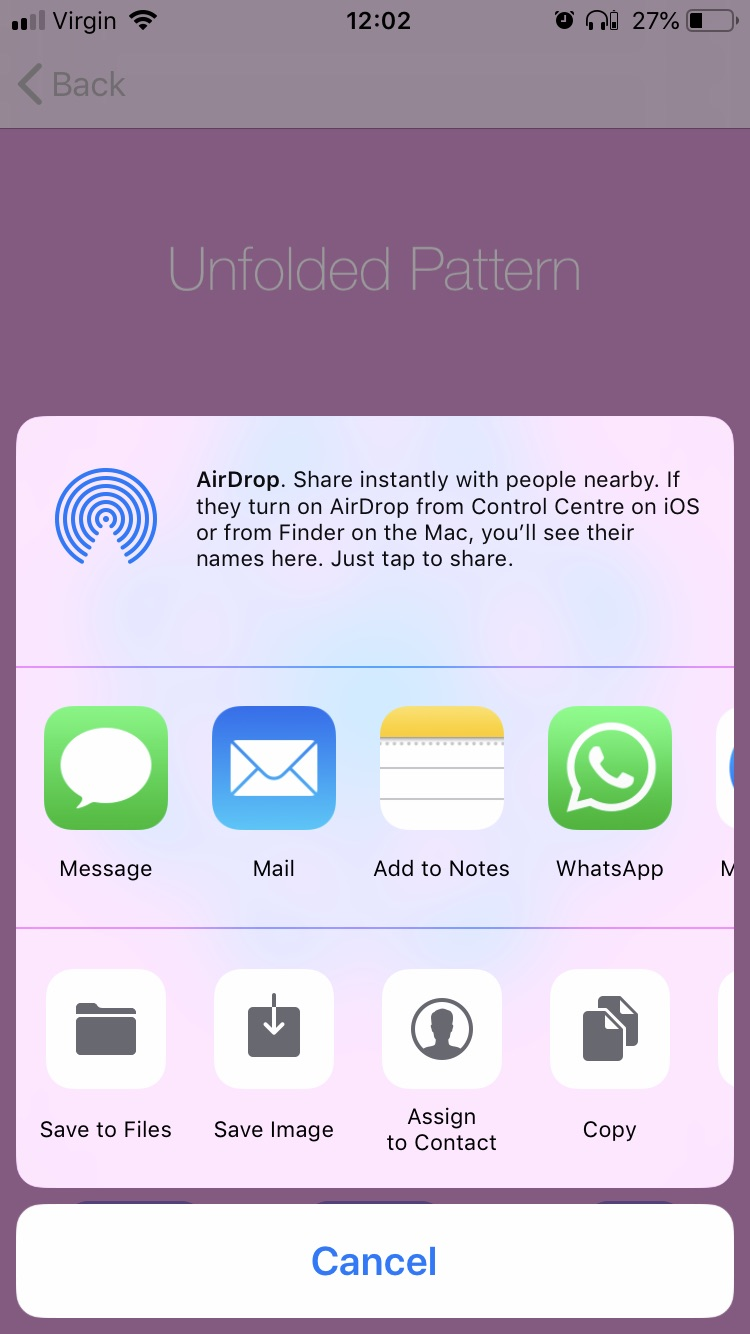
\includegraphics[width=0.7\linewidth]{KiriZen/share.jpeg}
                            \caption{The built in UI Activity View Controller the user can interact with to share the pattern they created on social media, messenger applications etc.}
                            \label{fig:kiriZen-share}
                        \end{minipage}\hfill
                        \begin{minipage}{0.45\textwidth}
                            \centering
                            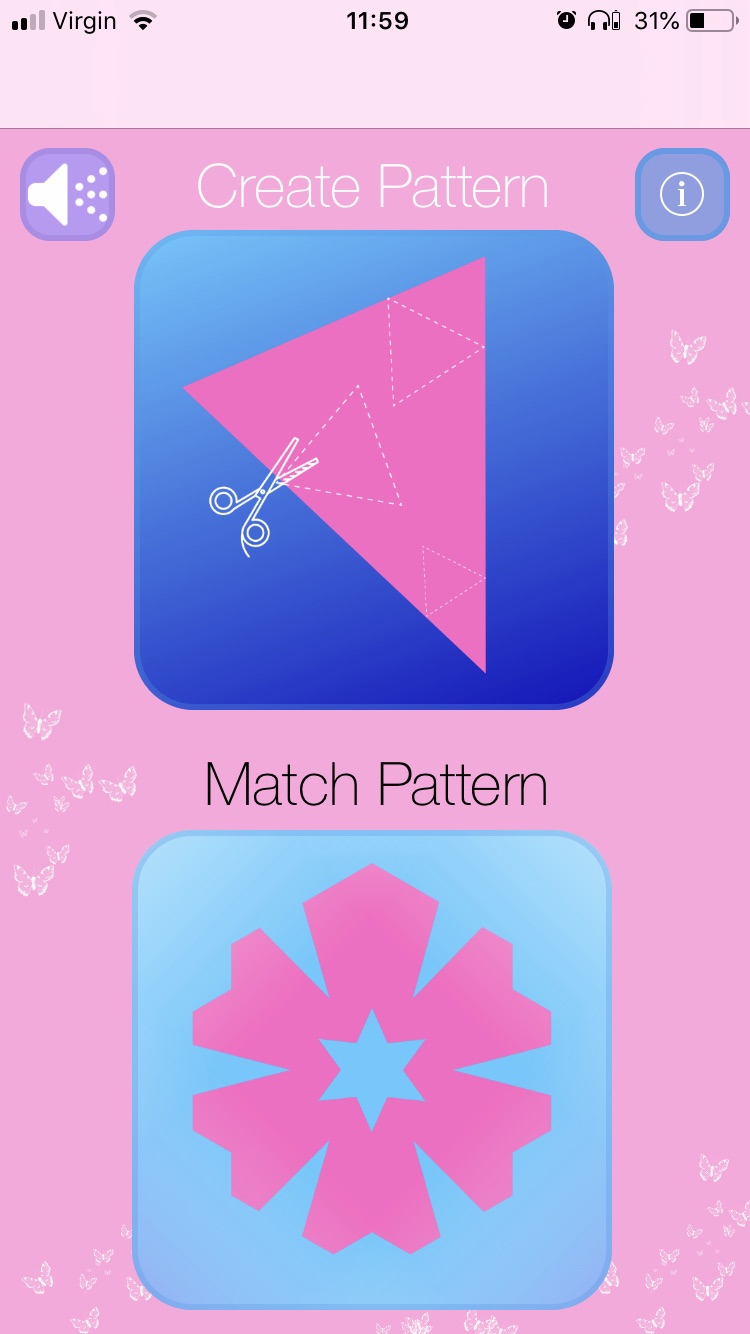
\includegraphics[width=0.7\linewidth]{KiriZen/main}
                            \caption{The home screen for the application with links to the information page, both parts of the app and the sound can be muted with the top left icon.}
                            \label{fig:kiriZen-main}
                        \end{minipage}
                    \end{figure}
                
                The share functionality was simple as there is a UI Activity View Controller (revealed in figure). Since the application does not contain sensitive information, I decided that there is no need to restrict the icons that appear in the view controller so the user is free to share their creation however they desire. The UI Activity View Controller is also a feature used in many applications so the user will be familiar with it and can interact seamlessly to share to their desired destination. The image shared has been cropped to just include the image of the unfolded paper and not the surrounding text or buttons. There was also feedback to include a print function which the user is able to do via this feature. The users responded very well to the save and share button as social media is such a major part of today's culture. I underestimated the positive response this feature would get.
            
             \subsubsection{Music Player}
                         \paragraph{}

                I found relaxing music from a free stock music website \cite{Lofi}  
                and contacted the creator to get permission to use it in KiriZen. I added the music to enhance the mindfulness aspect of the application.
                
                There is a mute button (shown in \textbf{Figure~\ref{fig:kiriZen-main}}) which changes to mute if clicked. To add the music I used an online tutorial \cite{MusicPlayer}.
                There are three ways to mute the music on my app. The two inbuilt speaker control buttons of the iPhone itself, this is to allow the user to mute the music how they would normally choose to in any other application. The third way is with the mute button on the applications home screen.
                
        \subsubsection{Instructions}
            
                \paragraph{}
                    The instructions page was initially one image which I updated to an animation as I noticed most users do not want to read the text.
                    As there was not much functionality to the information page, I mainly used the storyboard in Xcode to create a scroll-able screen (shown in \textbf{Figure~\ref{fig:kiriZen-instructionsCreate}} and \textbf{Figure~\ref{fig:kiriZen-instructionsMatch}}), however I coded the animation of the images using a timer to change the image every 0.4 seconds to the next one in the corresponding array. 
           
               \begin{figure}[!ht]
                                \begin{minipage}{0.45\textwidth}
                                    \centering 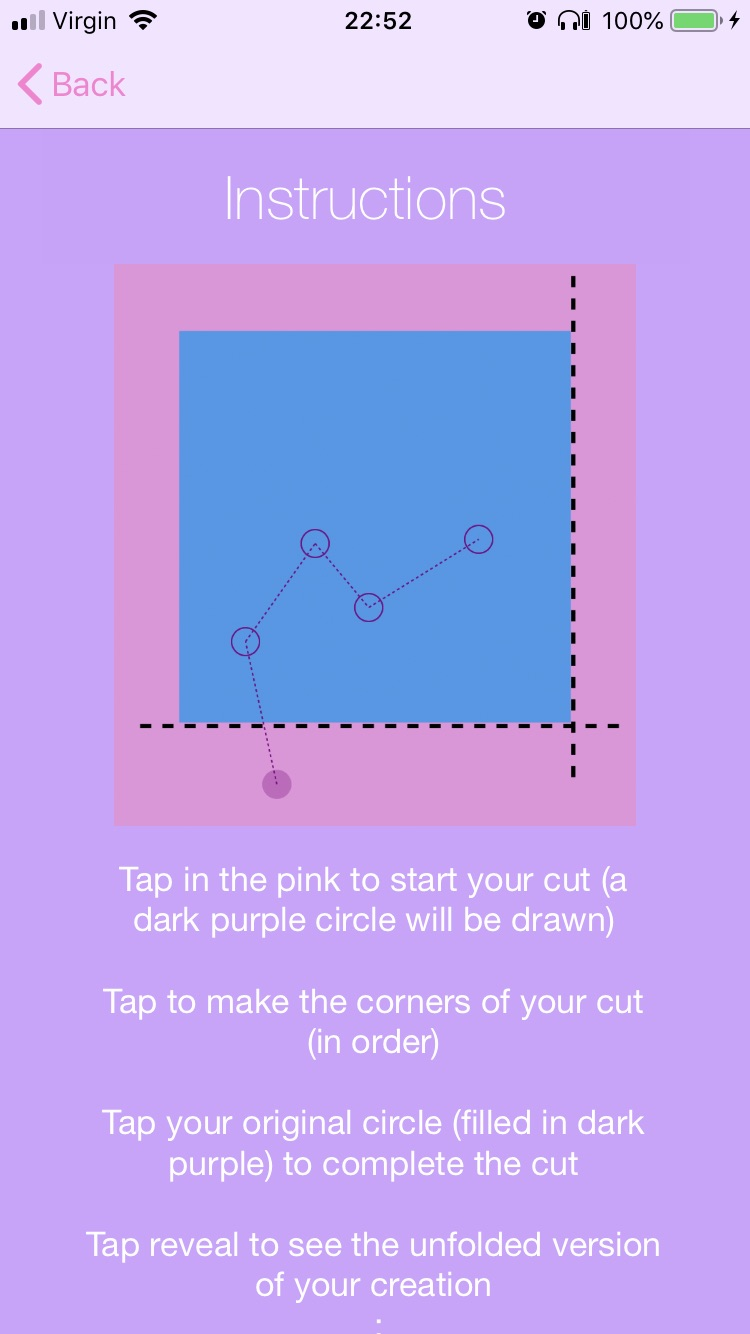
\includegraphics[width=0.7\linewidth]{KiriZen/instructionsCreate}
                                    \caption{The instructions for the ``Create Pattern" portion of the app. The image is animated showing how to cut from the virtual paper.}
                                    \label{fig:kiriZen-instructionsCreate}
                                \end{minipage}\hfill
                                \begin{minipage}{0.45\textwidth}
                                    \centering
                                    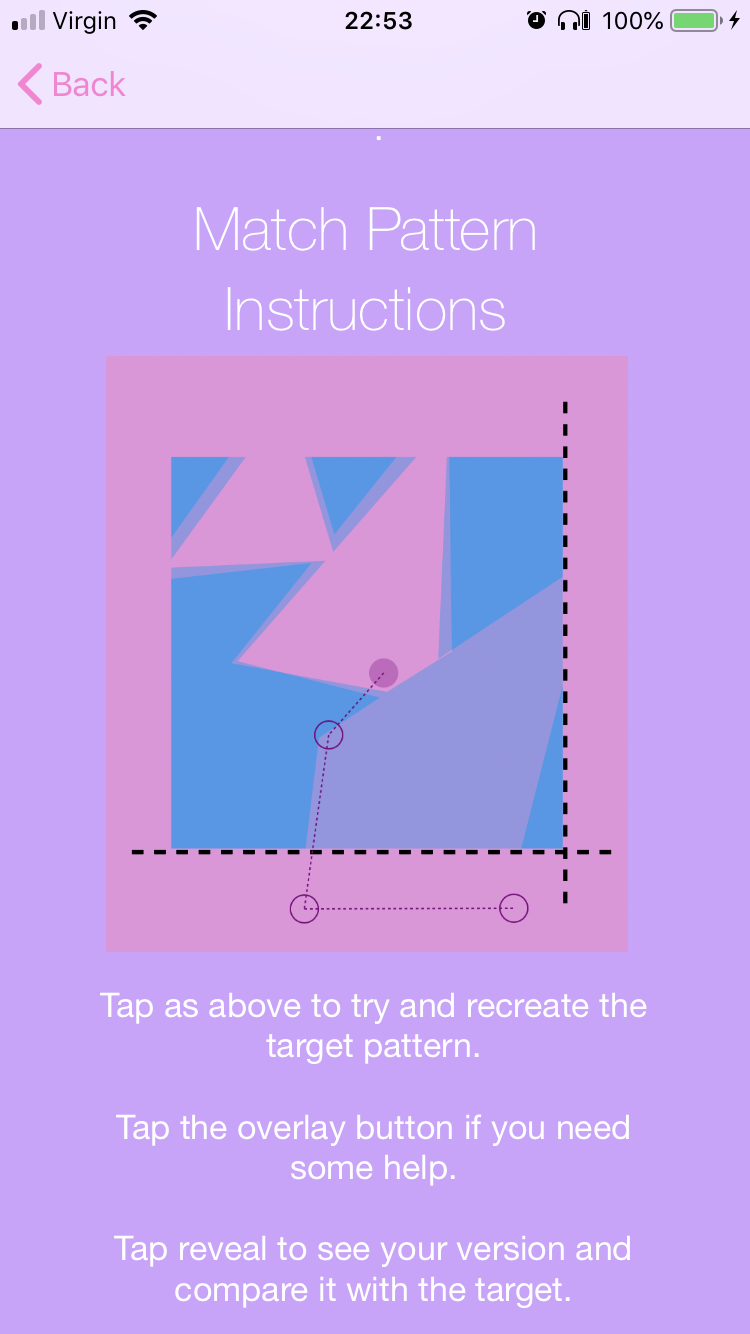
\includegraphics[width=0.7\linewidth]{KiriZen/instructionsMatch}
                                    \caption{The user can scroll down from the  \textbf{Figure~\ref{fig:kiriZen-instructionsCreate}} instructions to see the ``Match Pattern" portion of the instructions. This image is also animated.}
                                    \label{fig:kiriZen-instructionsMatch}
                                \end{minipage}
                            \end{figure}


                 \subsubsection{Launch Screen and Information Page}

                    \begin{figure}[!ht]
                        \begin{minipage}{0.45\textwidth}
                            \centering 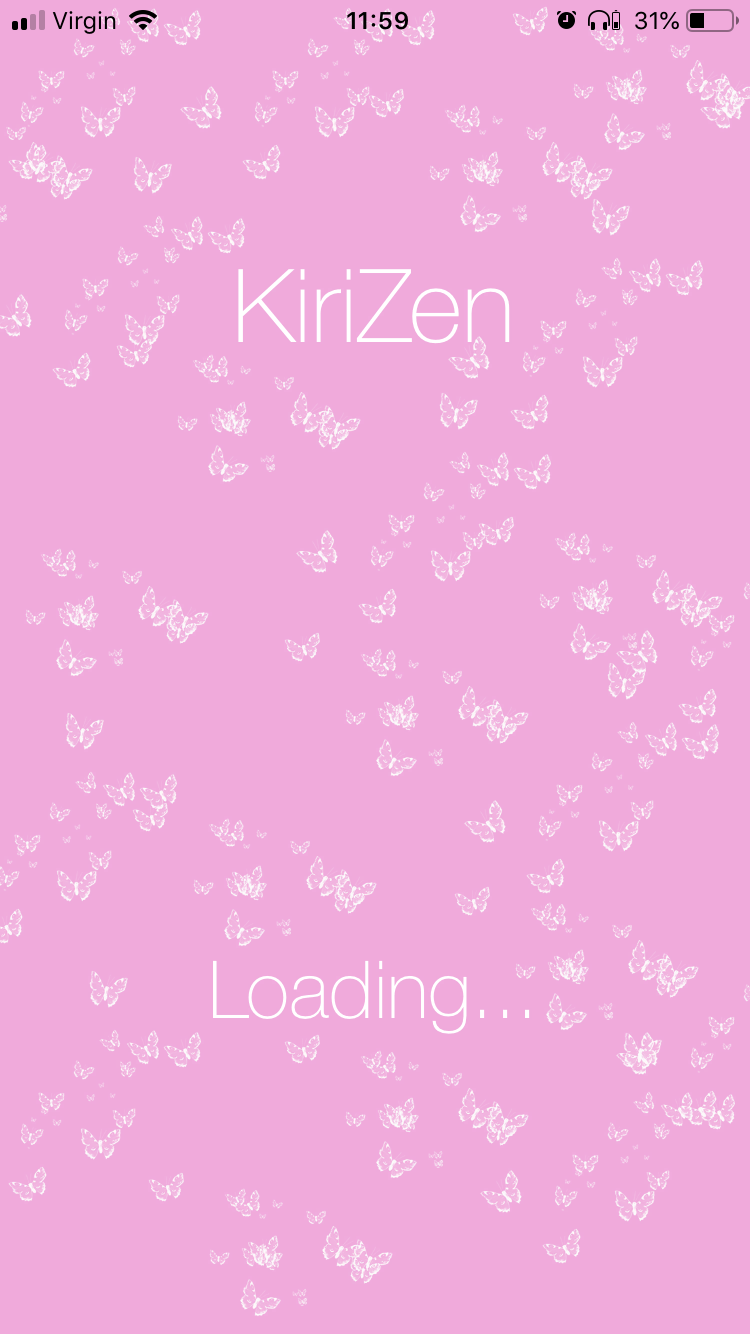
\includegraphics[width=0.7\linewidth]{KiriZen/launchPage}
                            \caption{The launch screen for the application that will appear while it is loading. The background reflects the theme and icon of the application.}
                            \label{fig:kiriZen-launch}
                        \end{minipage}\hfill
                        \begin{minipage}{0.45\textwidth}
                            \centering
                            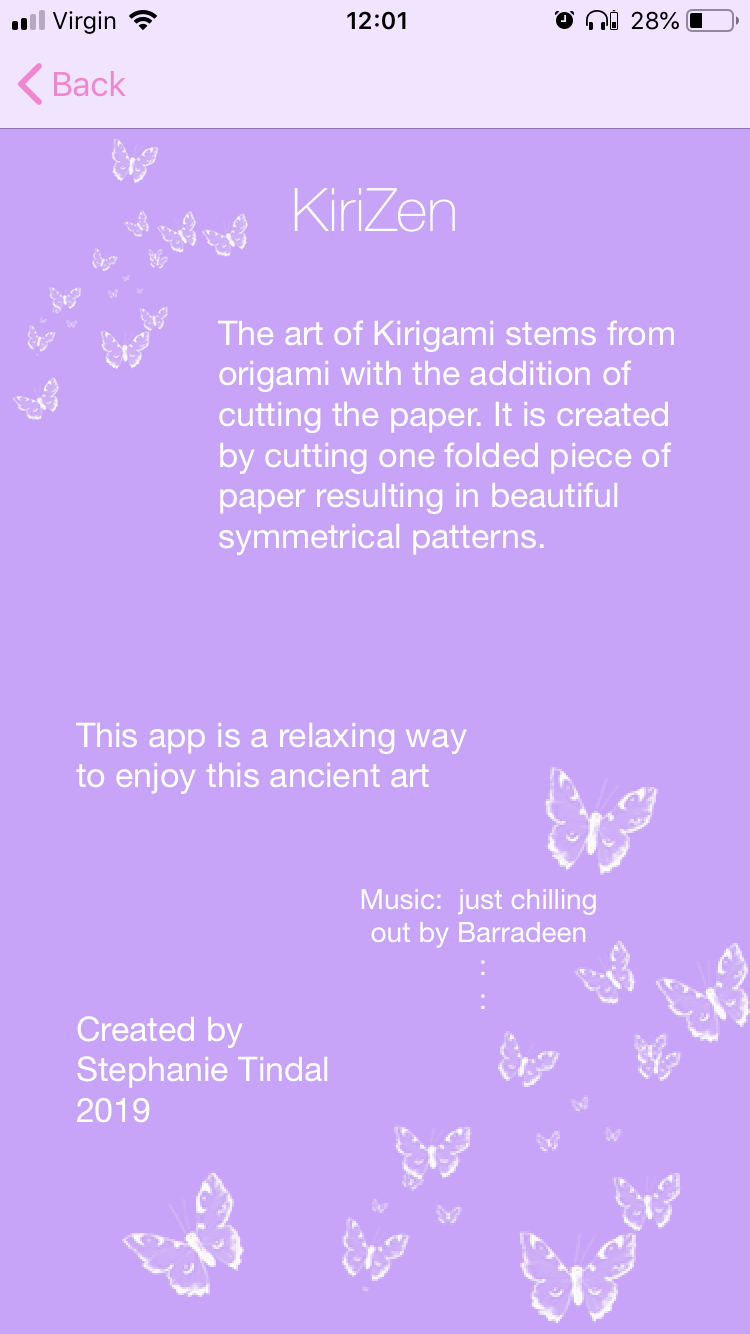
\includegraphics[width=0.7\linewidth]{KiriZen/info}
                            \caption{The information page linked from the info button in \textbf{Figure~\ref{fig:kiriZen-main}}.\\\\}
                            \label{fig:kiriZen-info}
                        \end{minipage}
                    \end{figure}
                    
                    \paragraph{}
                    I incorporated a loading screen (\textbf{Figure~\ref{fig:kiriZen-launch}}) for while the application is starting up so the user can view a page that is relevant to the application rather than the default white page. This is especially important if the application is taking a long time to open (usually this happens on the initial load if the application is not already running in the background). The butterflies on this page are in keeping with the theme and I have scattered them throughout the rest of the application too.
                    
                    The information page serves as insight for the user if they would like some additional information about the application and kirigami.
               
               \subsection{User Testing}
    
           \paragraph{Size}
           Throughout the project I asked my peers to test out the app and I observed how they interacted with it. For example, I observed that other users had larger hands and fingers than mine so the application was harder to interact with. I addressed this issue by enlarging the button size, and the radius of the initial circle so they do not have to be as precise when ending the cut. In addition to this, I was informed by the users that the icons on the initial screen were very small when side by side so I made the decision to enlarge them and stack them vertically to see the icon image more clearly. 
           
           \paragraph{Undo and Clear Functionality}
           I observed the user interacting with app and at first I only had the undo and clear buttons delete the cut shapes. However I noticed that the users also wanted this function while drawing their shape to edit their last point. After I incorporated this additional ``Undo" functionality, I observed new users interact with the application and they appeared to use this functionality with ease which I took to imply this functionality is expected. 
           
           \paragraph{Cutting the Shapes}
           Some more feedback that was provided by the users was that they would like lines between the circles so they can see the outline of the shape they are drawing before it is finalised, rather than imagining the lines. I added lines with small dashes to illustrate that this is where the cuts will occur and the users responded positively to this. 
           
            \subsection{Evaluation}
            
                \paragraph{}
                I used Nielsen's heuristics to conduct a usability overview. I used three evaluators and their responses are included in Appendix A. I asked the users to talk me through their comments so I could fully understand the problems. I gathered the information below to evaluate usability problems and suggested how to alleviate them \cite{Neil}.

                
                \paragraph{Visibility of system status}
                The application generally keeps users informed as to the status of their actions. For example, the buttons show a response. The addition of pop-ups indicate to the user that they should start cutting was suggested. 
                
                \paragraph{Match between system and real world}
                The functionality of the buttons is clear. The application is fairly realistic.
                
                \paragraph{User control and freedom}
                The in built navigation allows users to escape the current screen easily. The undo and clear allows the users to edit their patterns as they go, easily and intuitively. 

                \paragraph{Consistency and standards}
                The buttons are in the same place in both parts of the application so the users do not have to search for their positions. The user interface creates cuts that are predictable. The theme is present throughout, due to colour scheme.

                \paragraph{Error prevention}
                Unauthorised actions such as users starting a cut from the inside of the virtual blue paper, are prevented. Users are able to undo both types of actions e.g. undo a shape if that was the last thing created or undo a circle and path (indicating a new point) if that was last. Clear button can reset the page. 

                \paragraph{Recognition Rather than Recall}
                The buttons are easily recognisable due to the icons in the main screen and choose fold sections. The words on the create pattern screen buttons make the application easy to use. 
                
                The users must remember to click on the original circle they made to complete the cut. The application could be updated to cut the shape as soon as the line crosses outside the paper. However this would make it more challenging for certain shapes, therefore the advice should be tested before a final decision is made.


                \paragraph{Flexibility and efficiency of use} 
                The users reported that the application was flexible and efficient. The majority of the buttons have a quick response time. The target button needs some indication that you need to hold it down.

                \paragraph{Minimalist design}
                The application is clear overall without clutter, making it easy to use. Users agreed the design is minimalistic. 

                \paragraph{Help error recovery}
                Errors did not occur while the users were testing the application. Errors that could occur would likely be associated with the save/ share feature.

                \paragraph{Help and documentation} 
                The animation is helpful and the user can understand what to do after reading it. One user suggested adding instructions to the home screen page and changing the ``i" button to an ``About" button.
                
                \subsubsection{Heuristics Conclusion}
                \paragraph{}
                A few pop-ups would increase the ease of use of the app and allow the user to learn how to use the app faster, e.g. ``Tap here" if the user does not start the cut within a few taps. I could try to figure out some ways the users can accelerate function such as cutting, undo etc. to increase flexibility and efficiency. 
                
                The mute button is an example of flexibility within the app most users did not mute the application while testing. In the future I could allow users to test the application for a longer period of time / throughout the week to test the mindfulness aspect of the application which is difficult to test and measure in a short testing period. 
                
                 I could edit the colours of buttons to group their functionality e,g, undo and clear of a different colour to the other buttons. I do this with the information and instructions button which are always blue as seen in \textbf{Figure~\ref{fig:kiriZen-createPattern}}).
                
                The overall reaction of the application was positive with minor edits necessary. All heuristics were passed by the evaluators. The highest numeric value given was ``2" which is associated with minor usability problem.
                
        

    \subsection{Publishing}
        \paragraph{}
        When I have sufficient funds, I could potentially publish this application on the App Store. Before this takes place, the code should be tested on the latest beta version of Xcode software as it will contain extra upcoming features I will be able to test it on the updates that will be released shortly in the future (this is the purpose of the beta version). I will test it on other iOS devices other than iPhone 7/8 and edit the application accordingly.
        
        I would need to decide whether I would like to charge users for the app, or make it free. I believe a free app is more appropriate, especially for the target users and I, myself would prefer an unpaid application. However, as discussed in background research I would need to make sure the advertisements do not disrupt the user experience. As my goal is to create an application that is relaxing for users to use and not to make money, I could consider taking away all advertisements and making the app completely free.
        
        I would need to test this on a greater variety of users to see if I have fully achieved what I aimed for with this application as it was mostly my peers.  I can publish the application as test version to get user feedback on websites such as TestFlight \cite{TestFlight}.
        I could then check the user reviews and make appropriate edits if necessary. 
        
        If I published the application near Christmas, I could incorporate seasonal marketing. For example, extra snowflake designs for the target patterns, falling snowflake animations and wallpapers could be used in order to attract users at that time of year.
        
\newpage
\section{Discussion}
    \subsection{Achievements}
        \paragraph{}
        I created an application from scratch in a new language I was not familiar with which was a daunting task. The majority of users reported that they felt relaxed whilst using the application, confirming that it can be used as an effective part of the mindfulness practice. The background research I produced turned out to be extremely useful throughout the project. Whilst carrying out my investigation, I was surprised with how few of the apps had a reliable cutting features and there were many inconsistencies throughout. The application I created is unlike these as the cutting features are predictable which was confirmed in the evaluation. The users also confirmed that the buttons and theme were consistent. I am satisfied that I implemented all of the major requirements successfully, and was able to make improvements through adding smaller non-core features.
        
        I successfully made use of inheritance in the match pattern section of the application to reuse code already created rather than repeating it. I created a common buttons class with methods that create a subset of features of the buttons. This kept all the buttons consistent and I did not have to repeat the code upon each creation of a button. I learnt that refactoring my code, especially in the reveal section, by creating a transform function, helped to make my code easier to read and reduced the quantity. Throughout my code, I named the variables carefully which made it very easy to understand my thought process and the progression of the function when I looked at a section of code after a longer period of time. 
        
    \subsection{Challenges}
    
        \paragraph{}
        It was very challenging to create this application as I was unfamiliar with how the iPhone collects data from user interactions and what can be done in real time. For example, I attempted a few other methods of cutting before settling on the method similar to that of Paper Snowflake Maker, which was the best method found in the background research. This trial and error slowed the process down, however, I had a contingency plan in place where I left some time to spare that could be filled if required. I had never coded in this language so it took a few weeks to get used to the syntax and discover what methods are available to use.
        
        I had trouble layering the shapes on the screen when I was using different formats, which is why I decided to make the majority of objects on screen CA shapes. I eventually understood how to layer the objects and when to rearrange them. CA shapes were very helpful when creating the revealed version of the folds, created from triangular segments, as I used them as a mask to crop the copies to a triangle.
        
        One limitation of the application is compatibility. The application will currently only perform on iPhone 7 or 8 (I thoroughly tested it on this as the evaluators used my phone to trial the app). This will be something I will need to keep in mind when creating an app in the future, as there are over 10 devices that this application could be available on, including other iPhone versions and iPads. I would need to thoroughly test it on each device before publishing the application. 
            
    \subsection{Future}
                \paragraph{}
                
                The heuristic evaluation identified potential areas for improvement. These include editing features, such as the target button, to ease use and creating pop-ups as pointers during users first use of the app. Further testing is necessary on a wider range of users and I can evaluate their responses which can result in edits to the application. 
                
                Additional functionality could be added to the app such as an algorithm to generate random target images shaped but more sophisticated than randomly rendering shapes. Some restrictions could apply such as shapes not overlapping, the size of shapes and the variety of shapes.
                
                There could also be easy, medium, and hard levels or a next button within the match button section so the user could move on if they wished. 
                
                Algorithms for comparing target images to the image the user created.

                When saving the final image, there could be options for creating a wallpaper. They could be created by repeating the pattern
                along the style of tessellations. 

\newpage
\section{Conclusion}
        
            \paragraph{}
            This project meets the aim of creating and developing a kirigami based application from scratch to a final product. KiriZen will allow a new audience to experience kirigami as a relaxing, recreational activity with the potential for users to be inspired to physically recreate their favourite designs, created within the app. I am grateful to have had the opportunity to undertake this project and enjoyed the creativity and freedom of control that came with making it. I intend to publish it on the app store in the future, to disseminate KiriZen to a wider audience. Taking on board future feedback, I plan to continue updating and improving the app to make KiriZen the very best it can be.

\newpage
\let\Section\section 
\def\section*#1{\Section{#1}}  
\bibliographystyle{IEEEtran}
    \bibliography{bibliography}
    
    \newpage
      \subsection{Required Section on Code Sources}
            
            Code is commented and includes references when applicable. 
            
            \paragraph{Adapted from other sources:\\\\}
           
            Music Player 
            
            Title: How To Add Background Music In Swift
            
            Author: Zero To App Store
            
            Date: - Unknown
            
            Last Accessed: 01/09/2019
            
            Availability: zerotoappstore.com/how-to-add-background-music-in-swift.html

            \paragraph{\\}
            
            getPixelAt() function - gets colour of pixel line 335 in Canvas
            
            Title: Swift 4, Xcode 9 - With a UIImageView Extension
            
            Author: Mark Moeykens
            
            Date: 28/11/2017 (Last edit)
            
            Last Accessed: 19/07/2019
            
            Availability:
            
            stackoverflow.com/questions/12770181/how-to-get-the-pixel-color-on-touch
            
            \paragraph{\\}
            
            didPinch() function - zooms the final image in, line 397 in Reveal
            
            Title: Swift 3 solution
            
            Author: RajeshKumar R
            
            Date: 30/04/2018(Last edit)
            
            Last Accessed: 28/08/2019
            
            Availability: stackoverflow.com/questions/30014241/uiimageview-pinch-zoom-swift
            
            \paragraph{Automatically generated:}
            AppDelegate.swift, however I did not use this class. 
            The majority of Info.plist is generated apart from the ``Privacy - Photo Library Usage Description" as mentioned above. 
    
    \newpage
\Section{Appendix A}
Numeric Score Values:

0 - Don’t agree that this is a usability problem

1 - Cosmetic problem 

2 - Minor usability problem

3 - Medium problem (users can adapt) 

4 - Major usability problem

5 - Usability catastrophe

    \begin{figure}[!ht]
            \centering
            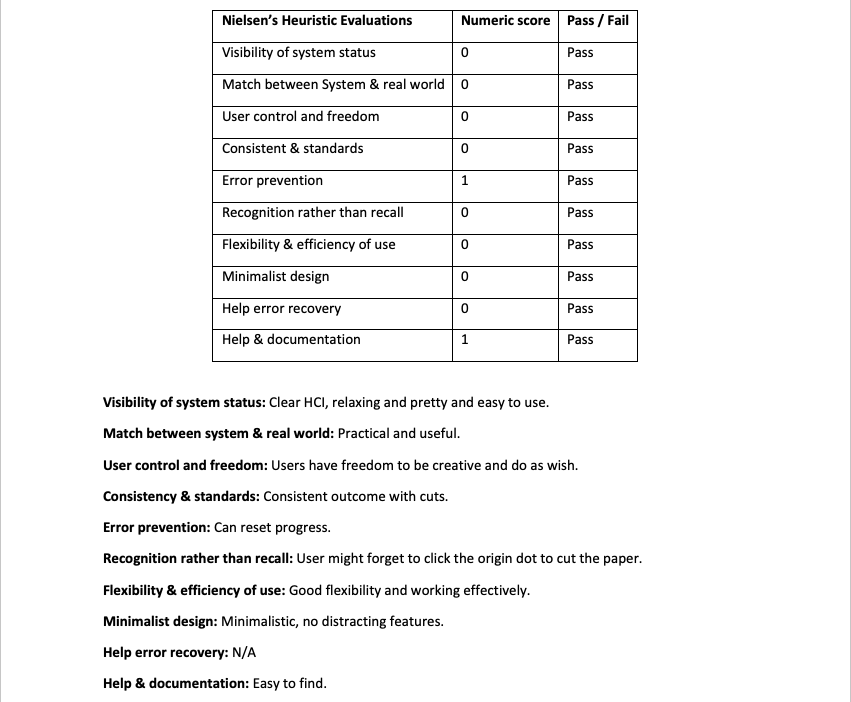
\includegraphics[width=1\linewidth]{Images/User1}
            \caption{The heuristics form for user 1.}
            \label{fig:user1}
    \end{figure}
    \begin{figure}[!ht]
            \centering
            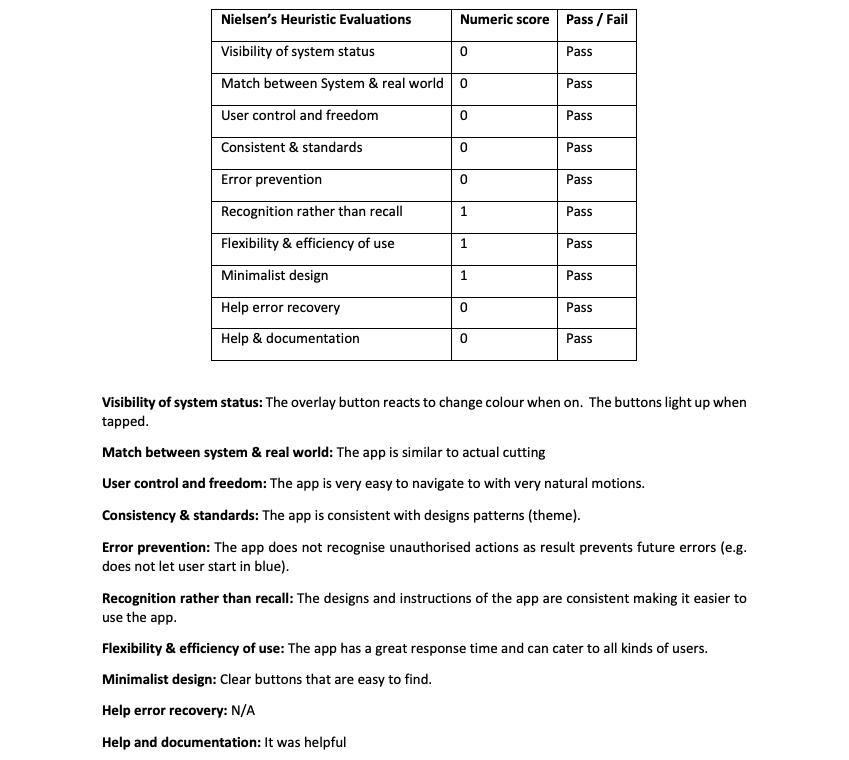
\includegraphics[width=1\linewidth]{Images/User2}
            \caption{The heuristics form for user 2.}
            \label{fig:user2}
    \end{figure}    
    \begin{figure}[!ht]
            \centering
            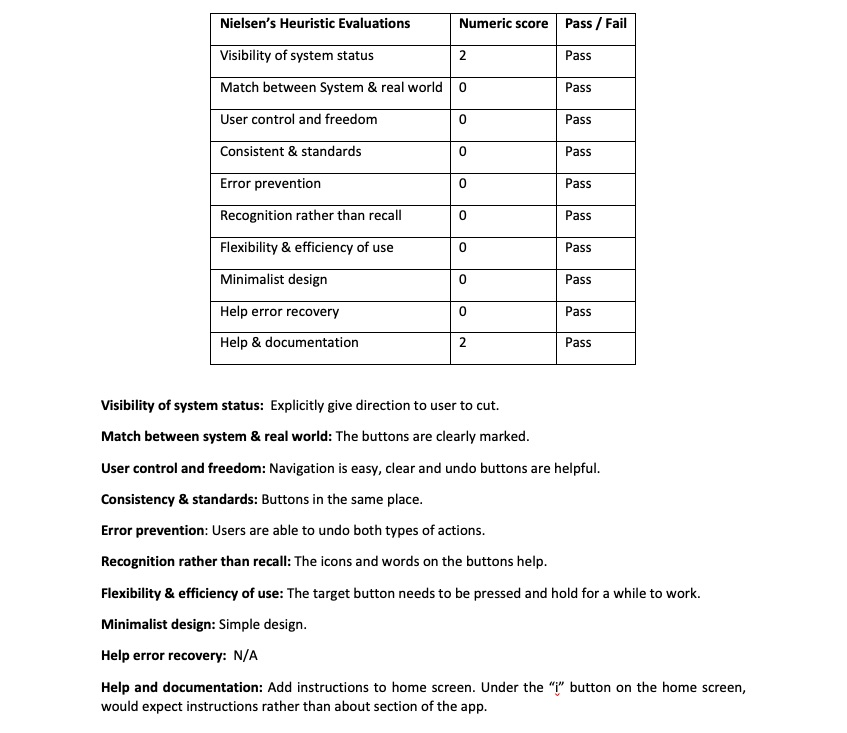
\includegraphics[width=1\linewidth]{Images/User3}
            \caption{The heuristics form for user 3.}
            \label{fig:user3}
    \end{figure}

\clearpage
\Section{Appendix B}

        \begin{enumerate}
            \item On a Mac running macOS 10.14.3 or later
            \item Download Xcode
            \item Download the project from 
            
            https://git-teaching.cs.bham.ac.uk/mod-msc-proj-2018/sct808
            \item Open ``kirigami draft 1.xcodeproj"
            \item Run on an iPhone 8 simmulator. 
            (It may not be possible to run on your own iPhone without already being an app developer, however an account can be created.)
      
        \end{enumerate}

\end{document}